% 若编译失败,且生成 .synctex(busy) 辅助文件,可能有两个原因:
% 1. 需要插入的图片不存在:Ctrl + F 搜索 'figure' 将这些代码注释/删除掉即可
% 2. 路径/文件名含中文或空格:更改路径/文件名即可

% --------------------- 文章宏包及相关设置 --------------------- %
% >> ------------------ 文章宏包及相关设置 ------------------ << %
% 设定文章类型与编码格式
\documentclass[UTF8]{article}		

% 物理实验报告所需的其它宏包
\usepackage{ulem}   % \uline 下划线支持
\usepackage{circuitikz} % 电路图 tikz 支持
\usepackage{pdfpages}   % 用于导入 pdf 文件
\usepackage{multirow}   % 用于表格合并单元格

% 本 .tex 专属的宏定义
    \def\V{\ \mathrm{V}}
    \def\uV{\ \mu\mathrm{V}}
    \def\mV{\ \mathrm{mV}}
    \def\K{\ \mathrm{K}}
    \def\kV{\ \mathrm{KV}}
    \def\KV{\ \mathrm{KV}}
    \def\MV{\ \mathrm{MV}}
    \def\uA{\ \mu\mathrm{A}}
    \def\mA{\ \mathrm{mA}}
    \def\A{\ \mathrm{A}}
    \def\kA{\ \mathrm{KA}}
    \def\KA{\ \mathrm{KA}}
    \def\MA{\ \mathrm{MA}}
    \def\O{\ \Omega}
    \def\mO{\ \Omega}
    \def\kO{\ \mathrm{K}\Omega}
    \def\KO{\ \mathrm{K}\Omega}
    \def\MO{\ \mathrm{M}\Omega}
    \def\Hz{\ \mathrm{Hz}}
    \def\uF{\ \mu\mathrm{F}}
    \def\mF{\ \mathrm{mF}}
    \def\F{\ \mathrm{F}}
    \def\Re{\mathrm{\,Re}\,}
    \def\Im{\mathrm{\,Im}\,}
    \def\sinc{\mathrm{\,sinc}\,}

% 自定义宏定义
    \def\N{\mathbb{N}}
    \def\F{\mathbb{F}}
    \def\Z{\mathbb{Z}}
    \def\Q{\mathbb{Q}}
    \def\R{\mathbb{R}}
    \def\C{\mathbb{C}}
    \def\T{\mathbb{T}}
    \def\S{\mathbb{S}}
    %\def\A{\mathbb{A}}
    \def\I{\mathscr{I}}
    \def\d{\mathrm{d}}
    \def\p{\partial}


% 导入基本宏包
    \usepackage[UTF8]{ctex}     % 设置文档为中文语言
    \usepackage{hyperref}  % 宏包:自动生成超链接 (此宏包与标题中的数学环境冲突)
    \hypersetup{
        colorlinks=true,    % false:边框链接 ; true:彩色链接
        citecolor={blue},    % 文献引用颜色
        linkcolor={blue},   % 目录 (我们在目录处单独设置),公式,图表,脚注等内部链接颜色
        urlcolor={orange},    % 网页 URL 链接颜色,包括 \href 中的 text
        % cyan 浅蓝色 
        % magenta 洋红色
        % yellow 黄色
        % black 黑色
        % white 白色
        % red 红色
        % green 绿色
        % blue 蓝色
        % gray 灰色
        % darkgray 深灰色
        % lightgray 浅灰色
        % brown 棕色
        % lime 石灰色
        % olive 橄榄色
        % orange 橙色
        % pink 粉红色
        % purple 紫色
        % teal 蓝绿色
        % violet 紫罗兰色
    }
    % \usepackage{docmute}    % 宏包:子文件导入时自动去除导言区,用于主/子文件的写作方式,\include{./51单片机笔记}即可。注:启用此宏包会导致.tex文件capacity受限。
    \usepackage{amsmath}    % 宏包:数学公式
    \usepackage{mathrsfs}   % 宏包:提供更多数学符号
    \usepackage{amssymb}    % 宏包:提供更多数学符号
    \usepackage{pifont}     % 宏包:提供了特殊符号和字体
    \usepackage{extarrows}  % 宏包:更多箭头符号 
    \usepackage{multicol}   % 宏包:支持多栏 

% 文章页面margin设置
    \usepackage[a4paper]{geometry}
        \geometry{top=0.75in}
        \geometry{bottom=0.75in}
        \geometry{left=0.75in}
        \geometry{right=0.75in}   % 设置上下左右页边距
        \geometry{marginparwidth=1.75cm}    % 设置边注距离(注释、标记等)

% 配置数学环境
    \usepackage{amsthm} % 宏包:数学环境配置
    % theorem-line 环境自定义
        \newtheoremstyle{MyLineTheoremStyle}% <name>
            {11pt}% <space above>
            {11pt}% <space below>
            {}% <body font> 默认使用正文字体,  为楷体
            {}% <indent amount>
            {\bfseries}% <theorem head font> 设置标题项为加粗
            {:\ \ }% <punctuation after theorem head>
            {.5em}% <space after theorem head>
            {\textbf{#1}\thmnumber{#2}\ \ (\,\textbf{#3}\,)}% 设置标题内容顺序
        \theoremstyle{MyLineTheoremStyle} % 应用自定义的定理样式
        \newtheorem{LineTheorem}{Theorem.\,}
    % theorem-block 环境自定义
        \newtheoremstyle{MyBlockTheoremStyle}% <name>
            {11pt}% <space above>
            {11pt}% <space below>
            {}% <body font> 使用默认正文字体
            {}% <indent amount>
            {\bfseries}% <theorem head font> 设置标题项为加粗
            {:\\ \indent}% <punctuation after theorem head>
            {.5em}% <space after theorem head>
            {\textbf{#1}\thmnumber{#2}\ \ (\,\textbf{#3}\,)}% 设置标题内容顺序
        \theoremstyle{MyBlockTheoremStyle} % 应用自定义的定理样式
        \newtheorem{BlockTheorem}[LineTheorem]{Theorem.\,} % 使用 LineTheorem 的计数器
    % definition 环境自定义
        \newtheoremstyle{MySubsubsectionStyle}% <name>
            {11pt}% <space above>
            {11pt}% <space below>
            {}% <body font> 使用默认正文字体
            {}% <indent amount>
            {\bfseries}% <theorem head font> 设置标题项为加粗
            {:\\ \indent}% <punctuation after theorem head>
            {0pt}% <space after theorem head>
            {\textbf{#3}}% 设置标题内容顺序
        \theoremstyle{MySubsubsectionStyle} % 应用自定义的定理样式
        \newtheorem{definition}{}

%宏包:有色文本框(proof环境)及其设置
    \usepackage{xcolor}    %设置插入的文本框颜色
    \usepackage[strict]{changepage}     % 提供一个 adjustwidth 环境
    \usepackage{framed}     % 实现方框效果
        \definecolor{graybox_color}{rgb}{0.95,0.95,0.96} % 文本框颜色。修改此行中的 rgb 数值即可改变方框纹颜色,具体颜色的rgb数值可以在网站https://colordrop.io/ 中获得。(截止目前的尝试还没有成功过,感觉单位不一样)(找到喜欢的颜色,点击下方的小眼睛,找到rgb值,复制修改即可)
        \newenvironment{graybox}{%
        \def\FrameCommand{%
        \hspace{1pt}%
        {\color{gray}\vrule width 2pt}%
        {\color{graybox_color}\vrule width 4pt}%
        \colorbox{graybox_color}%
        }%
        \MakeFramed{\advance\hsize-\width\FrameRestore}%
        \noindent\hspace{-4.55pt}% disable indenting first paragraph
        \begin{adjustwidth}{}{7pt}%
        \vspace{2pt}\vspace{2pt}%
        }
        {%
        \vspace{2pt}\end{adjustwidth}\endMakeFramed%
        }

% 外源代码插入设置
    % matlab 代码插入设置
    \usepackage{matlab-prettifier}
        \lstset{style=Matlab-editor}    % 继承 matlab 代码高亮 , 此行不能删去
    \usepackage[most]{tcolorbox} % 引入tcolorbox包 
    \usepackage{listings} % 引入listings包
        \tcbuselibrary{listings, skins, breakable}
        \newfontfamily\codefont{Consolas} % 定义需要的 codefont 字体
        \lstdefinestyle{MatlabStyle_inc}{   % 插入代码的样式
            language=Matlab,
            basicstyle=\footnotesize\ttfamily\codefont,    % ttfamily 确保等宽 
            breakatwhitespace=false,
            breaklines=true,
            captionpos=b,
            keepspaces=true,
            numbers=left,
            numbersep=15pt,
            showspaces=false,
            showstringspaces=false,
            showtabs=false,
            tabsize=2,
            xleftmargin=15pt,   % 左边距
            %frame=single, % single 为包围式单线框
            frame=shadowbox,    % shadowbox 为带阴影包围式单线框效果
            %escapeinside=``,   % 允许在代码块中使用 LaTeX 命令 (此行无用)
            %frameround=tttt,    % tttt 表示四个角都是圆角
            framextopmargin=0pt,    % 边框上边距
            framexbottommargin=0pt, % 边框下边距
            framexleftmargin=5pt,   % 边框左边距
            framexrightmargin=5pt,  % 边框右边距
            rulesepcolor=\color{red!20!green!20!blue!20}, % 阴影框颜色设置
            %backgroundcolor=\color{blue!10}, % 背景颜色
        }
        \lstdefinestyle{MatlabStyle_src}{   % 插入代码的样式
            language=Matlab,
            basicstyle=\small\ttfamily\codefont,    % ttfamily 确保等宽 
            breakatwhitespace=false,
            breaklines=true,
            captionpos=b,
            keepspaces=true,
            numbers=left,
            numbersep=15pt,
            showspaces=false,
            showstringspaces=false,
            showtabs=false,
            tabsize=2,
        }
        \newtcblisting{matlablisting}{
            %arc=2pt,        % 圆角半径
            % 调整代码在 listing 中的位置以和引入文件时的格式相同
            top=0pt,
            bottom=0pt,
            left=-5pt,
            right=-5pt,
            listing only,   % 此句不能删去
            listing style=MatlabStyle_src,
            breakable,
            colback=white,   % 选一个合适的颜色
            colframe=black!0,   % 感叹号后跟不透明度 (为 0 时完全透明)
        }
        \lstset{
            style=MatlabStyle_inc,
        }

% table 支持
    \usepackage{booktabs}   % 宏包:三线表
    \usepackage{tabularray} % 宏包:表格排版
    \usepackage{longtable}  % 宏包:长表格

% figure 设置
    \usepackage{graphicx}  % 支持 jpg, png, eps, pdf 图片 
    \usepackage{svg}       % 支持 svg 图片
        \svgsetup{
            % 指向 inkscape.exe 的路径
            inkscapeexe = C:/aa_MySame/inkscape/bin/inkscape.exe, 
            % 一定程度上修复导入后图片文字溢出几何图形的问题
            inkscapelatex = false                 
        }
    \usepackage{subcaption} % 用于子图和小图注  

% 图表进阶设置
    \usepackage{caption}    % 图注、表注
        \captionsetup[figure]{name=图}  
        \captionsetup[table]{name=表}
        \captionsetup{
            labelfont=bf, % 设置标签为粗体
            textfont=bf,  % 设置文本为粗体
            font=small  
        }
    \usepackage{float}     % 图表位置浮动设置 
    \usepackage{etoolbox} % 用于保证图注表注的数学字符为粗体
        \AtBeginEnvironment{figure}{\boldmath} % 图注中的数学字符为粗体
        \AtBeginEnvironment{table}{\boldmath}  % 表注中的数学字符为粗体
        \AtBeginEnvironment{tabular}{\unboldmath}   % 保证表格中的数学字符不受额外影响

% 圆圈序号自定义
    \newcommand*\circled[1]{\tikz[baseline=(char.base)]{\node[shape=circle,draw,inner sep=0.8pt, line width = 0.03em] (char) {\bfseries #1};}}   % TikZ solution

% 列表设置
    \usepackage{enumitem}   % 宏包:列表环境设置
        \setlist[enumerate]{
            label=(\arabic*) ,   % 设置序号样式为加粗的 (1) (2) (3)
            ref=\arabic*, % 如果需要引用列表项,这将决定引用格式(这里仍然使用数字)
            itemsep=0pt, parsep=0pt, topsep=0pt, partopsep=0pt, leftmargin=3.5em} 
        \setlist[itemize]{itemsep=0pt, parsep=0pt, topsep=0pt, partopsep=0pt, leftmargin=3.5em}
        \newlist{circledenum}{enumerate}{1} % 创建一个新的枚举环境  
        \setlist[circledenum,1]{  
            label=\protect\circled{\arabic*}, % 使用 \arabic* 来获取当前枚举计数器的值,并用 \circled 包装它  
            ref=\arabic*, % 如果需要引用列表项,这将决定引用格式(这里仍然使用数字)
            itemsep=0pt, parsep=0pt, topsep=0pt, partopsep=0pt, leftmargin=3.5em
        }  

% 其它设置
    % 脚注设置
        \renewcommand\thefootnote{\ding{\numexpr171+\value{footnote}}}
    % 参考文献引用设置
        \bibliographystyle{unsrt}   % 设置参考文献引用格式为unsrt
        \newcommand{\upcite}[1]{\textsuperscript{\cite{#1}}}     % 自定义上角标式引用
    % 文章序言设置
        \newcommand{\cnabstractname}{序言}
        \newenvironment{cnabstract}{%
            \par\Large
            \noindent\mbox{}\hfill{\bfseries \cnabstractname}\hfill\mbox{}\par
            \vskip 2.5ex
            }{\par\vskip 2.5ex}

% 文章默认字体设置
    \usepackage{fontspec}   % 宏包:字体设置
        \setmainfont{SimSun}    % 设置中文字体为宋体字体
        \setCJKmainfont[AutoFakeBold=3]{SimSun} % 设置加粗字体为 SimSun 族,AutoFakeBold 可以调整字体粗细
        \setmainfont{Times New Roman} % 设置英文字体为Times New Roman

% 各级标题自定义设置
    \usepackage{titlesec}   
        % section标题自定义设置 
        \titleformat{\section}[hang]{\normalfont\Large\bfseries\boldmath}{\thesection}{8pt}{}
        % subsection 标题自定义设置
        \titleformat{\subsection}[hang]{\normalfont\large\bfseries\boldmath}{\thesubsection}{8pt}{}
        \titlespacing*{\subsection}{0pt}{10pt}{6pt} % 控制上下间距


% --------------------- 文章宏包及相关设置 --------------------- %
% >> ------------------ 文章宏包及相关设置 ------------------ << %


% ------------------------ 文章信息区 ------------------------ %
% ------------------------ 文章信息区 ------------------------ %

% 每次实验报告需要修改的信息有:
% 1. 左上角页眉
% 2. 实验名称
% 3. 实验日期
% 4. 实验地点
% 5. 指导教师

% 页眉页脚设置
\usepackage{fancyhdr}   %宏包:页眉页脚设置
    \pagestyle{fancy}
    \fancyhf{}
    \cfoot{\thepage}
    \renewcommand\headrulewidth{1pt}
    \renewcommand\footrulewidth{0pt}
    \rhead{\bfseries \large {\color{red} 分组序号: 2-05}}
    \chead{《基础物理实验》实验报告,\ 丁毅,\ 2023K8009908031}
    \lhead{\small Ex.06 谐振电路 (2024.12.24)}
\begin{document}


\begin{center}\large
    \vspace*{-0.6cm}
    \noindent{\huge\bfseries《\ \ 基\ \ 础\ \ 物\ \ 理\ \ 实\ \ 验\ \ \ 》\ \ 实\ \ 验\ \ 报\ \ 告 }
    \\\vspace{0.3cm}
    \noindent{
    {\bfseries 
    实验名称:\uline{\hspace{0.6cm} $RLC$ 电路的谐振与暂态过程 \hspace{0.6cm}}
    }\hspace{0.2cm}
    指导教师:\uline{\hspace{0.2cm}邓体建 \  \ dengtijian@ihep.ac.cn \hspace{0.2cm}}
    }
    \\\vspace{0.1cm}
    \noindent
    {
    姓名:\uline{\,\,\,丁毅\,\,\,}\hspace{0.2cm}
    学号:\uline{\,\,\,{ 2023K8009908031}\,\,\,}\hspace{0.2cm}
    班级/专业:\uline{\,\,\,{2308/电子信息}\,\,\,}\hspace{0.2cm}
    分组序号:\uline{\,\,\,{2-05}\,\,\,}
    }
    \\\vspace{0.1cm}
    \noindent{
    实验日期:\uline{\,\,{ 2024.12.24}\,\,}\hspace{0.2cm}
    实验地点:\uline{\,\,\,教学楼{709}\,\,\,}\hspace{0.2cm}
    是否调课/补课:\uline{\hspace{0.26cm}否 \hspace{0.26cm}}\hspace{0.2cm}
    成绩:\uline{\hspace{2cm}}
    }
\end{center}
\vspace{-0.3cm}
\noindent\rule{\textwidth}{0.075em}   % 分割线
\vspace{-1.1cm}

% 目录
%\zihao{-5}
\setcounter{tocdepth}{3}  % 目录深度为 2(不显示 subsubsection)
\noindent\tableofcontents\thispagestyle{fancy}   % 显示页码、页眉等
\newpage
\rhead{\bfseries\small 分组序号: 2-05}
\zihao{5}
% ------------------------ 文章信息区 ------------------------ %
% ------------------------ 文章信息区 ------------------------ %


%% 下面是正文内容

\section{实验目的}
\begin{enumerate}
\item 通过观察示波器中的波形研究$ RLC $电路的谐振现象。
\item 了解$ RLC $电路的相频特性与振幅特性。
\item 通过示波器中的波形观察$ RLC $串联电路的暂态过程。
\end{enumerate}


\section{实验仪器与用具}
标准电感、标准电容,$ 100\,\Omega $标准电阻,电阻箱,电感箱,函数发生器,示波器,数字多用表,导线等。

\section{实验原理}
\subsection{$ RLC $串联谐振电路}
\begin{figure}[H]
    \centering
    \begin{circuitikz}
        \draw (6,0)
        to[sV,a=$ \tilde u_s $] (0,0)
        to[short] (0,-3)
        to[european resistor,l=$ R $] (2,-3)
        to[american inductor,l=$ L $] (4,-3)
        to[C,l=$ C $] (6,-3)
        to[short] (6,0);
        \draw[->] (5,0)--(5.1,0)node[above]{$ \tilde i $};
        \draw[<-] (0.1,-1.5)--(2.7,-1.5);
        \draw[->] (3.3,-1.5)--(5.9,-1.5);
        \node at(3,-1.5) {$ \tilde u $};
        \draw (6,-3.5)--(6,-4.5);
        \draw (4,-3.5)--(4,-4.5);
        \draw (2,-3.5)--(2,-4.5);
        \draw (0,-3.5)--(0,-4.5);
        \draw[<-] (0.05,-4)--(0.7,-4);
        \draw[<-] (2.05,-4)--(2.7,-4);
        \draw[<-] (4.05,-4)--(4.7,-4);
        \draw[->] (1.3,-4)--(1.95,-4);
        \draw[->] (3.3,-4)--(3.95,-4);
        \draw[->] (5.3,-4)--(5.95,-4);
        \node at(1,-4) {$ \tilde u_R $};
        \node at(3,-4) {$ \tilde u_L $};
        \node at(5,-4) {$ \tilde u_C $};
    \end{circuitikz}
    \caption{$ RLC $串联谐振电路}
\end{figure}

$ RLC $串联谐振电路如上图所示,利用复数法\footnote{本实验报告中复数法记法约定$ \tilde x $表示复变量,$ x $表示其模长,虚单位为$ j=\sqrt{-1} $。}分析电路可求得电容$ C $、电感$ L $、电阻$ R $的复阻抗分别为
\begin{equation}
\tilde{Z}_C=\frac{1}{j\omega C},\quad \tilde{Z}_L=j\omega L,\quad\tilde{Z}_R=R
\end{equation}
进而可求得电路的总复阻抗与总阻抗:
\begin{equation}
\tilde{Z}=R+j\left(\omega L-\frac{1}{\omega C}\right)\,\Longrightarrow\,Z=\left|\tilde{Z}\right|=\sqrt{R^2+\left(\omega L-\frac{1}{\omega C}\right)^2}
\end{equation}
电流$ i $的大小为
\begin{equation}
i=\frac uZ=\frac{1}{\sqrt{R^2+\left(\omega L-\frac{1}{\omega C}\right)^2}}
\end{equation}
路端电压$ u $与电流$ i $的相位差为
\begin{equation}
\varphi=\arctan\frac{\omega L-\frac{1}{\omega C}}{R}
\end{equation}
以上诸式中$ \omega=2\pi f $为交变电压$ u $的角频率,$ f $为其频率。可见$ Z,\,\varphi,i $均为$ f $的函数,即当电路中其他元件参量确定的情况下,电路特性将完全取决于频率的大小。


\subsubsection{呈纯电阻性}

当$ \Im \tilde{Z}=0 $,即$ \omega L-\frac{1}{\omega C}=0 $时,总阻抗呈电阻性,且总阻抗达到最小值$ Z_0=R $,电压与电路的相位差$ \varphi=0 $,电流达到最大值$ i_{\max}=\frac uR $,这种状态称为串联谐振。此时的角频率$ \omega_0 $称为谐振角频率,相应地此时频率$ f_0 $称为谐振频率,其具体大小为
\begin{equation}
\omega_0=\frac{1}{\sqrt{LC}},\quad f_0=\frac{1}{2\pi\sqrt{LC}}
\end{equation}
谐振时,有
\begin{equation}
u_L=i_{\max} Z_L=\frac{\omega_0L}{R}u,\quad \frac{u_L}{u}=\frac{\omega_0L}{R}=\frac1R\sqrt{\frac LC}
\end{equation}
而
\begin{equation}
u_C=i_{\max} Z_C=\frac{u}{R\omega_0C},\quad\frac{u_C}{u}=\frac{1}{R\omega_0C}=\frac1R\sqrt{\frac LC}
\end{equation}
令
\begin{equation}
Q=\frac{u_L}{u}=\frac{u_C}{u}=\frac{\omega_0L}{R}=\frac{1}{R\omega_0C}
\end{equation}
$ Q $称为谐振电路的品质因数,是标志和衡量谐振电路性能优劣的重要参量。$ Q $可衡量的电路性能有:
\begin{enumerate}
\item 储耗能特性:$ Q $值越大,相对的储能耗能越小,储能效率越高;
\item 电压分配特性:串联谐振时$ u_L=u_C=Qu $,电感、电容上的电压均为输入电压的$ Q $倍,因此有时称串联谐振为电压谐振。利用电压谐振,可在某些传感器、信息接收中显著提高灵敏度或效率,但在某些应用场合,它对系统和人员却具有一定不安全性,故而在设计与操作中应予以注意。
\item 频率选择性:设$ f_1,\;f_2 $为谢振峰两侧$ i=\frac{i_{\max}}{\sqrt 2} $处对应频率,则$ \Delta f=f_2-f_1 $称为通频带宽度,简称带宽。不难证明有
\end{enumerate}


\begin{equation}
Q=\frac{f_0}{\Delta f}
\end{equation}
当$ Q $值越大时,带宽越窄,峰越尖锐,频率选择性越好。

\subsubsection{呈感性}

当$ \Im \tilde{Z}>0 $,即$ \omega L-\frac{1}{\omega C}>0 $时,总阻抗呈电感性,此时电压与电流相位差$ \varphi>0 $,交变电压频率$ f>f_0 $,并且随着$ f $的增大,$ \varphi $趋近于$ \frac\pi2 $,阻抗越大,电流越小。

\subsubsection{呈容性}

当$ \Im \tilde{Z}<0 $,即$ \omega L-\frac{1}{\omega C}<0 $时,总阻抗呈电感性,此时电压与电流相位差$ \varphi<0 $,交变电压频率$ f<f_0 $,并且随着$ f $的减小,$ \varphi $趋近于$ -\frac\pi2 $,阻抗越大,电流越小。

\subsection{$ RLC $并联谐振电路}
\begin{figure}[H]
    \centering
    \begin{circuitikz}
        \draw (6,0)
        to[sV,a=$ \tilde u_s $] (0,0)
        to[short] (0,-1.5)
        to[european resistor,l=$ R' $,-*] (2,-1.5)
        to[european resistor,l=$ R $] (4,-1.5)
        to[american inductor,l=$ L $,-*] (6,-1.5)
        to[short,-.] (6,0);
        \draw (2,-1.5)
        to[short] (2,-3)
        to[C,l=$ C $] (6,-3)
        to[short] (6,-1.5);
        
        \draw[->] (5,0)--(5.1,0)node[above]{$ \tilde i $};
        \draw[<-] (5.7,-1.5)node[above]{$ \tilde i_L $}--(5.8,-1.5);
        \draw[<-] (5.5,-3)node[above]{$ \tilde i_C $}--(5.6,-3);
        
        \draw (0,-3.5)--(0,-4.5);
        \draw (2,-3.5)--(2,-4.5);
        \draw (6,-3.5)--(6,-4.5);
        \draw[<-] (0.05,-4)--(0.7,-4);
        \draw[->] (1.3,-4)--(1.95,-4);
        \node at(1,-4) {$ \tilde u_{R'} $};
        \draw[<-] (2.05,-4)--(3.7,-4);
        \draw[->] (4.3,-4)--(5.95,-4);
        \node at(4,-4) {$ \tilde u $};
    \end{circuitikz}
    \caption{$ RLC $并联谐振电路}
\end{figure}

利用复数法分析上图电路,电容$ C $、电感$ L $、电阻$ R $的复阻抗分别为
\begin{equation}
\tilde{Z}_C=\frac{1}{j\omega C},\quad\tilde{Z}_L=j\omega L,\quad \tilde{Z}_R=R
\end{equation}
那么电路并联部分的总复阻抗为
\begin{equation}
\tilde{Z}_p=\frac{1}{j\omega C+\frac{1}{R+j\omega L}}=\frac{R+j\omega L}{(1-\omega^2LC)+j\omega CR}
\end{equation}
从而可求得电路并联部分总电阻为
\begin{equation}
Z_p=\left|\tilde{Z}_p\right|=\sqrt{\frac{R^2+(\omega R)^2}{(1-\omega^2LC)^2+(\omega CR)^2}}
\end{equation}
并联部分电压$ u $与干路电流$ i $的相位差为
\begin{equation}
\varphi=\arctan\frac{\omega L-\omega C[R^2+(\omega L)^2]}{R}
\end{equation}
并联部分电压$ u $大小为
\begin{equation}
u=iZ_p=\frac{u_{R'}}{R'}Z_p
\end{equation}

\begin{enumerate}
\item 当$ \Im \tilde{Z}_p=0 $,即$ \varphi=0 $时,总阻抗呈纯电阻性,可求得其并联谐振的角频率$ \omega_p $与频率$ f_p $为
\begin{equation}
\omega_p=\sqrt{\frac{1}{LC}-\left(\frac RL\right)^2}=\omega_0\sqrt{1-\frac{1}{Q^2}},\quad f_p=\frac{1}{2\pi}\sqrt{\frac{1}{LC}-\left(\frac RL\right)^2}
\end{equation}
即并联谐振频率$ f_p $与串联谐振频率$ f_0 $稍有不同,当$ Q\gg 1 $时,$ \omega_p\approx\omega_0 $,$ f_p\approx f_0 $。

\item 当$ f<f_p $时,$ \varphi>0 $,电流相位落后于电压,整个电路呈电感性。

\item 当$ f>f_p $时,$ \varphi<0 $,电流相位超前于电压,整个电路呈电容性。
\end{enumerate}


在谐振频率两侧区域,并联电路的电抗特性与串联电路相反。在$ f=f_p' $\footnote{$ f_p' $与$ f_p $稍有不同。}处总阻抗达到极大值,总电流达到极小值。而在$ f_p' $两侧,随$ f $偏离$ f_p' $越远,阻抗越小,电流越大。

与串联谐振类似,可用品质因数
\begin{equation}
Q_1=\frac{\omega_0L}{R}=\frac{1}{R\omega_0C},\quad Q_2=\frac{i_C}{i}\approx\frac{i_L}{i},\quad Q_3=\frac{f_0}{\Delta f}
\end{equation}
来标志并联谐振电路的性能优劣,有时也称并联谐振为电流谐振。

\subsection{$ RLC $电路的暂态过程}
\begin{figure}[H]
    \centering
    \begin{circuitikz}
        \draw (0,2)
        to[battery1,a=$ E $] (0,0)
        to[short,-*] (1.5,0)
        to[short] (2,0)
        to[american inductor,a=$ L $] (5,0)
        to[C,l=$ C $] (5,2)
        to[european resistor,a=$ R $,-.] (2,2);
        \draw[thick] (2,2)node[above left]{$ S $}--(1.3,1.6);
        \draw (1.5,0)
        to[short] (1.5,1.6)node[right]{2};
        \draw (0,2)
        to[short,.-] (1.3,2)node[above]{1};
        \draw (5.5,0)--(6.5,0);
        \draw (5.5,2)--(6.5,2);
        \draw[<-] (6,0.05)--(6,0.7);
        \draw[->] (6,1.3)--(6,1.95);
        \node at(6,1) {$ u_C $};
    \end{circuitikz}
    \caption{$ RLC $串联振荡电路}
\end{figure}

在$ RLC $串联振荡电路中,开关拨向不同的端口,电路呈现为两种状态:当开关$ S $拨向1时,电源$ E $接入电路,为电容$ C $进行充电;当开关$ S $拨向2时,电容在$ RLC $串联电路中放电。在放电过程中,根据实际电路可列出常微分方程
\begin{equation}
L\frac{\mathrm{d} i}{\mathrm{d} t}+Ri+u_C=0
\end{equation}
电容存储的电荷量$ q=Cu_C $,那么电路中的电流为
\begin{equation}
i=\frac{\mathrm{d} q}{\mathrm{d} t}=C\frac{\mathrm{d} u_C}{\mathrm{d} t}
\end{equation}
将其代入电路常微分方程即得到关于$ u_C $的二阶齐次常微分方程
\begin{equation}
LC\frac{\mathrm{d}^2u_C}{\mathrm{d} t^2}+RC\frac{\mathrm{d} u_C}{\mathrm{d} t}+u_C=0
\end{equation}
考虑初始条件即可得到方程组:
\begin{equation}
\begin{cases}
    LC\dfrac{\mathrm{d}^2u_C}{\mathrm{d} t^2}+RC\dfrac{\mathrm{d} u_C}{\mathrm{d} t}+u_C=0\\
    u_C=E\qquad(t=0)\\
    C\dfrac{\mathrm{d} u_C}{\mathrm{d} t}=0\qquad(t=0)
\end{cases}
\end{equation}
引入阻尼系数$ \zeta=\frac R2\sqrt{\frac CL} $,则可将方程组的解分为三种情况:

\subsubsection{欠阻尼}

当$ \zeta<1 $,即$ R^2<\frac{4L}{C} $时,阻尼不足,上述方程组的解为
\begin{equation}
u_C=\sqrt{\frac{4L}{4L-R^2C}}E\,e^{-t/\tau}\cos(\omega t+\varphi)
\end{equation}
其中时间常量$ \tau=\frac{2L}{R} $,衰减振动的角频率为$ \omega=\frac{1}{\sqrt{LC}}\sqrt{1-\frac{R^2C}{4L}} $。$ \tau $的大小决定了振幅衰减的快慢,$ \tau $越小,振幅衰减越迅速。

若$ R^2\ll\frac{4L}{C} $,振幅的衰减很缓慢,此时
\begin{equation}
\omega\approx\frac{1}{\sqrt{LC}}=\omega_0
\end{equation}
近似为$ LC $电路自由振动,$ \omega_0 $为$ R=0 $时$ LC $回路的固有频率。衰减振动的周期为
\begin{equation}
T=\frac{2\pi}{\omega}\approx2\pi\sqrt{LC}
\end{equation}


\subsubsection{过阻尼}
当$ \zeta>1 $,即$ R^2>\frac{4L}{C} $时,对应过阻尼状态,方程组的解为
\begin{equation}
u_C=\sqrt{\frac{4L}{R^2C-4L}}E\,e^{-\alpha t}\sinh(\beta t+\varphi)
\end{equation}
其中$ \alpha=\frac{R}{2L},\;\beta=\frac{1}{\sqrt{LC}}\sqrt{\frac{R^2C}{4L}-1} $。此时振幅将缓慢地衰减为0。若固定$ L,\;C $。

\subsubsection{临界阻尼}

当$ \zeta=1 $,即$ R^2=\frac{4L}{C} $时,对应临界阻尼状态,方程组的解为
\begin{equation}
u_C=E\left(1+\frac t\tau\right)\,e^{-t/\tau}
\end{equation}
其中$ \tau=\frac{2L}{R} $,其为从过阻尼到阻尼振动过渡的分界点。

对于充电过程,考虑初始条件,电路方程组变为
\begin{equation}
\begin{cases}
    LC\dfrac{\mathrm{d}^2u_C}{\mathrm{d} t^2}+RC\dfrac{\mathrm{d} u_C}{\mathrm{d} t}+u_C=E\\
    u_C=0\qquad(t=0)\\
    \dfrac{\mathrm{d} u_C}{\mathrm{d} t}=0\qquad(t=0)
\end{cases}
\end{equation}

\subsubsection{充电过程微分方程的解}

当$ R^2<\frac{4L}{C} $时,方程组的解为
\begin{equation}
u_C=E\left[1-\sqrt{\frac{4L}{4L-R^C}}\,e^{-t/\tau}\cos(\omega t+\varphi)\right]
\end{equation}

当$ R^2>\frac{4L}{C} $时,方程组的解为
\begin{equation}
u_C=E\left[1-\sqrt{\frac{4L}{R^2C-4L}}\,e^{-\alpha t}\sinh(\beta t+\varphi)\right]
\end{equation}

当$ R^2=\frac{4L}{C} $时,方程组的解为
\begin{equation}
u_C=E\left[1-\left(1+\frac t\tau\right)\,e^{-t/\tau}\right]
\end{equation}

可以看出,充电过程与放电过程十分类似,只是最后趋向的平衡位置不同。

\section{实验内容}
\subsection{测$ RLC $串联电路的相频特性曲线和幅频特性曲线}
取$ u_{pp}=2.0\,\mathrm V,\;L=0.1\,\mathrm H,\;C=0.05\,\mu\mathrm F,\;R=100\,\Omega $时,用示波器CH1、CH2通道分别观测$ RLC $串联电路的总电压$ u $和电阻两端电压$ u_R $。注意限制总电压峰值不超过$ 3.0\,\mathrm V $(或有效值不超过0.1\,V),防止串联谐振时产生有危险的高电压。

1.调谐振,改变函数发生器的输出频率,通过CH1与CH2相位差为0,CH2幅度最大来判断谐振与否,记录谐振时的频率$ f_0 $.

2.用万用表记录谐振时的电感、电容两端的电压$ u_L,\;u_C $,和电源路端电压$ u $并计算$ Q $值。

3.保持CH1的幅度为$ 2\,\mathrm V $不变,按照建议的频率点测量CH1与CH2的相位差、CH2的幅度值,并绘制相频曲线和幅频曲线,即$ \varphi-f $图像、$ i-f $图像。

\subsection{测$ RLC $并联电路的相频特性和幅频特性曲线}
取$ u+u_{R'}=2.0\,\mathrm V,\;L=0.1\,\mathrm H,\;C=0.05\,\mu\mathrm F,\;R'=5\,\mathrm k\Omega $。为观测电感与电容并联部分的电压和相位,用CH1测量总电压,用CH2测量$ R' $两端电压,两通道测量电压值相减即为并联部分的电压$ u $,可通过示波器面板上的“MATH”键实现两通道波形相减。

1.调节函数发生器频率,通过观察CH1$ - $CH2与CH2相位差为0,CH2的幅度最小来判断谐振点,记录此时的频率。

2.保持CH1总电压幅度值2\,V不变(不同频率点需要调节函数发生器),按照建议的频率点测量CH1$ - $CH2与CH2的相位差,与CH1$ - $CH2、CH2的幅度值,绘制相频曲线与幅频曲线,即$ \varphi-f $图像、$ i-f $图像、$ u-f $图像。

\subsection{观测$ RLC $串联电路的暂态过程}
由函数发生器产生方波,为便于观察,需将方波的低电平调整至与示波器的扫描基线一致。由低电平到高电平相当于充电,由高电平到低电平相当于放电。函数发生器各参数可设置为:频率50\,Hz,电压峰峰值$ u_{pp}=2.0\,\mathrm V $,偏移1\,V。示波器CH1通道用于测量总电压,CH2用来测量电容两端电压$ u_C $,注意两个通道必须共地。实验中$ L=0.1\,\mathrm H,\;C=0.2\,\mu\mathrm F $.

1.当$ R=0\,\Omega $时,测量$ u_C $波形;

2.调节$ R $测得临界电阻$ R_C $,并与理论值比较;

3.记录$ R=2\,\mathrm{k}\Omega,\;20\,\mathrm k\Omega $的$ u_C $波形。函数发生器频率可设置为250\,Hz($ R=2\,\mathrm k\Omega $)和20\,Hz($ R=20\,\mathrm k\Omega $).

\section{实验结果与数据处理}

\begin{graybox}
    本次实验中,除了完成实验规定的测量、记录任务,我们还额外用自带的 Analog Discovery 1 (后文简称“AD1”) 设备测量了更为完整的阻抗与相位曲线,以及电压与电流的波形。我们会在后文依次给出两者的测量结果。
\end{graybox}

\subsection{测$ RLC $串联电路的相频特性曲线和幅频特性曲线}
根据实验电路的参数可计算得到$ Q $的理论标准值
\begin{equation}
Q=\frac1R\sqrt\frac LC = 14.142
\end{equation}

调节函数发生器输出频率,当$ f=2.2475\,\mathrm{kHz} $时,路端电压与电阻$ R $两端电压相位差趋近为 0,达到串联谐振状态,此时用数字多用表测得
\begin{equation}
U_{RMS} = 0.463 \ \mathrm{V},\quad
U_{C, RMS} = 5.50 \ \mathrm{V},\quad 
U_{L, RMS} = 5.52 \ \mathrm{V},\quad
\end{equation}
故而可计算得到电路的品质因数,理论与实际值对比如下:
\begin{table}[H]\centering
    %\renewcommand{\arraystretch}{1.5} % 调整行间距为 1.5 倍
    %\setlength{\tabcolsep}{1.5mm} % 调整列间距
    \caption{$ RLC $ 串联谐振频率与品质因子}
\begin{tabular}{cccccccccc}\toprule
    $f_{\text{expe}}$ & $f_{\text{theo}}$ & $U_{RMS}$ & $U_{C, RMS}$ & $U_{L, RMS}$ & $Q_{\text{theo}}$ & $Q_{\text{expe}}$ \\
    \midrule
    2.2475 KHz & 2.2508 KHz &  0.463 V & 5.50 V & 5.52 V & 14.1421 & 11.9006 \\
    \bottomrule
\end{tabular}
\end{table}

在实验讲义给出的参考频率下,保证路端电压$ u_{pp}=2.0\,\mathrm V $不变的情况下测得电压、电流相位差,以及相应的$ u_R $值记录如表 \ref{RLC 串联谐振电路实验数据记录} 。

\begin{table}[H]\centering
    %\renewcommand{\arraystretch}{1.5} % 调整行间距为 1.5 倍
    %\setlength{\tabcolsep}{1.5mm} % 调整列间距
    \caption{$ RLC $ 串联谐振电路实验数据记录}
    \label{RLC  串联谐振电路实验数据记录}
\begin{tabular}{cccccccccc}\toprule
    $f$ (KHz) & $U_{\text{amp}}$ (V) & $\varphi$ ($^\circ$) & $U_{R, \text{amp}}$ (mV) & $I_{\max}$ (mA)  \\
    \midrule
    1.88	&2.00	&-87.23	&12.6	&0.13   \\
    2.00	&2.00	&-85.82	&81.1	&0.81   \\
    2.08	&2.00	&-83.58	&215	&2.15   \\
    2.15	&2.00	&-78.90	&523	&5.23   \\
    2.19	&2.00	&-70.30	&950	&9.50   \\
    2.22	&2.00	&-62.11	&1190	&11.90  \\
    2.24	&2.00	&-23.06	&1560	&15.60  \\
    2.25	&2.00	&8.79	&1590	&15.90  \\
    2.26	&2.00	&29.79	&1540	&15.40  \\
    2.275	&2.00	&53.98	&1330	&13.30  \\
    2.30	&2.00	&68.89	&992	&9.92   \\
    2.36	&2.00	&79.75	&457	&4.57   \\
    2.43	&2.00	&83.43	&211	&2.11   \\
    2.62	&2.00	&86.57	&32.5	&0.33   \\
    3.18	&2.00	&88.12	&11.4	&0.11   \\
    \bottomrule
\end{tabular}
\end{table}

根据数据记录可作出$ \varphi-f,\;i-f $图像如下。

\begin{figure}[H]\centering
\begin{subfigure}[b]{0.5\columnwidth}\centering
    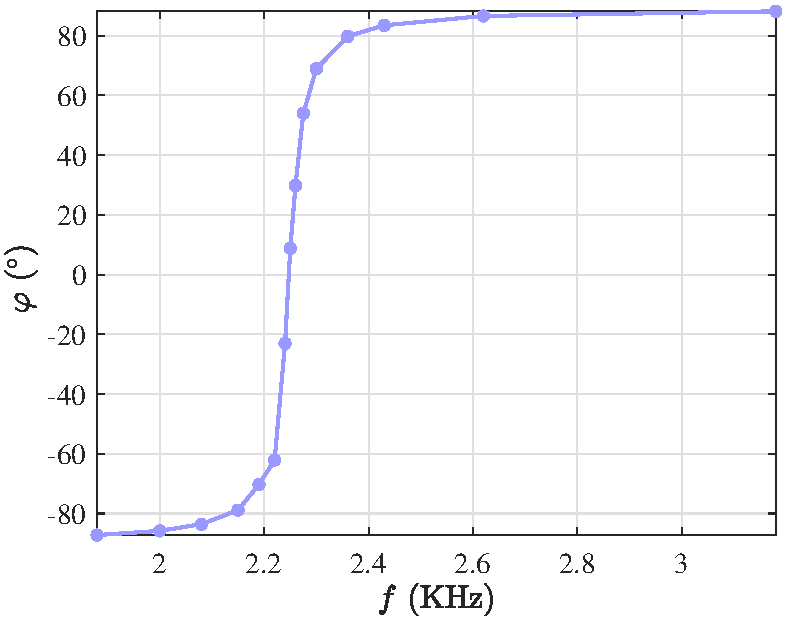
\includegraphics[height=180pt]{assets/1/2024-12-24_22-29-46.pdf}
    \caption{相位 $\varphi$}
\end{subfigure}\hfill
\begin{subfigure}[b]{0.5\columnwidth}\centering
    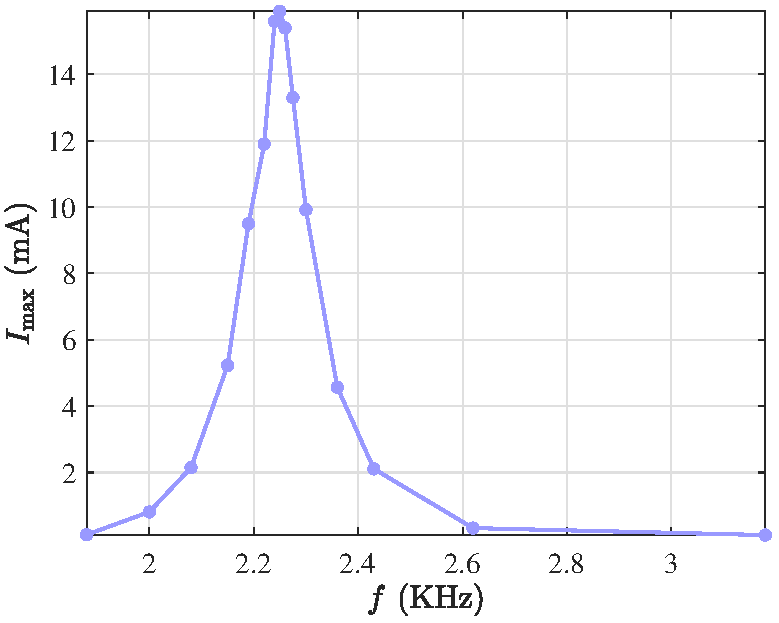
\includegraphics[height=180pt]{assets/1/2024-12-24_22-29-49.pdf}
    \caption{电流 $I_{\max}$}
\end{subfigure}
\caption{$RLC$ 串联电路频率响应}
\end{figure}
由$ i-f $图像可读得谐振频率为$ f_0=2.247\,\mathrm{kHz} $,通频带宽为$ \Delta f = 0.182\,\mathrm{kHz} $,故而可算得品质因子
\begin{equation}
Q'=\frac{f_0}{\Delta f} = 12.3462
\end{equation}

用 AD1 测得阻抗与相位曲线如下:
\begin{figure}[H]\centering
    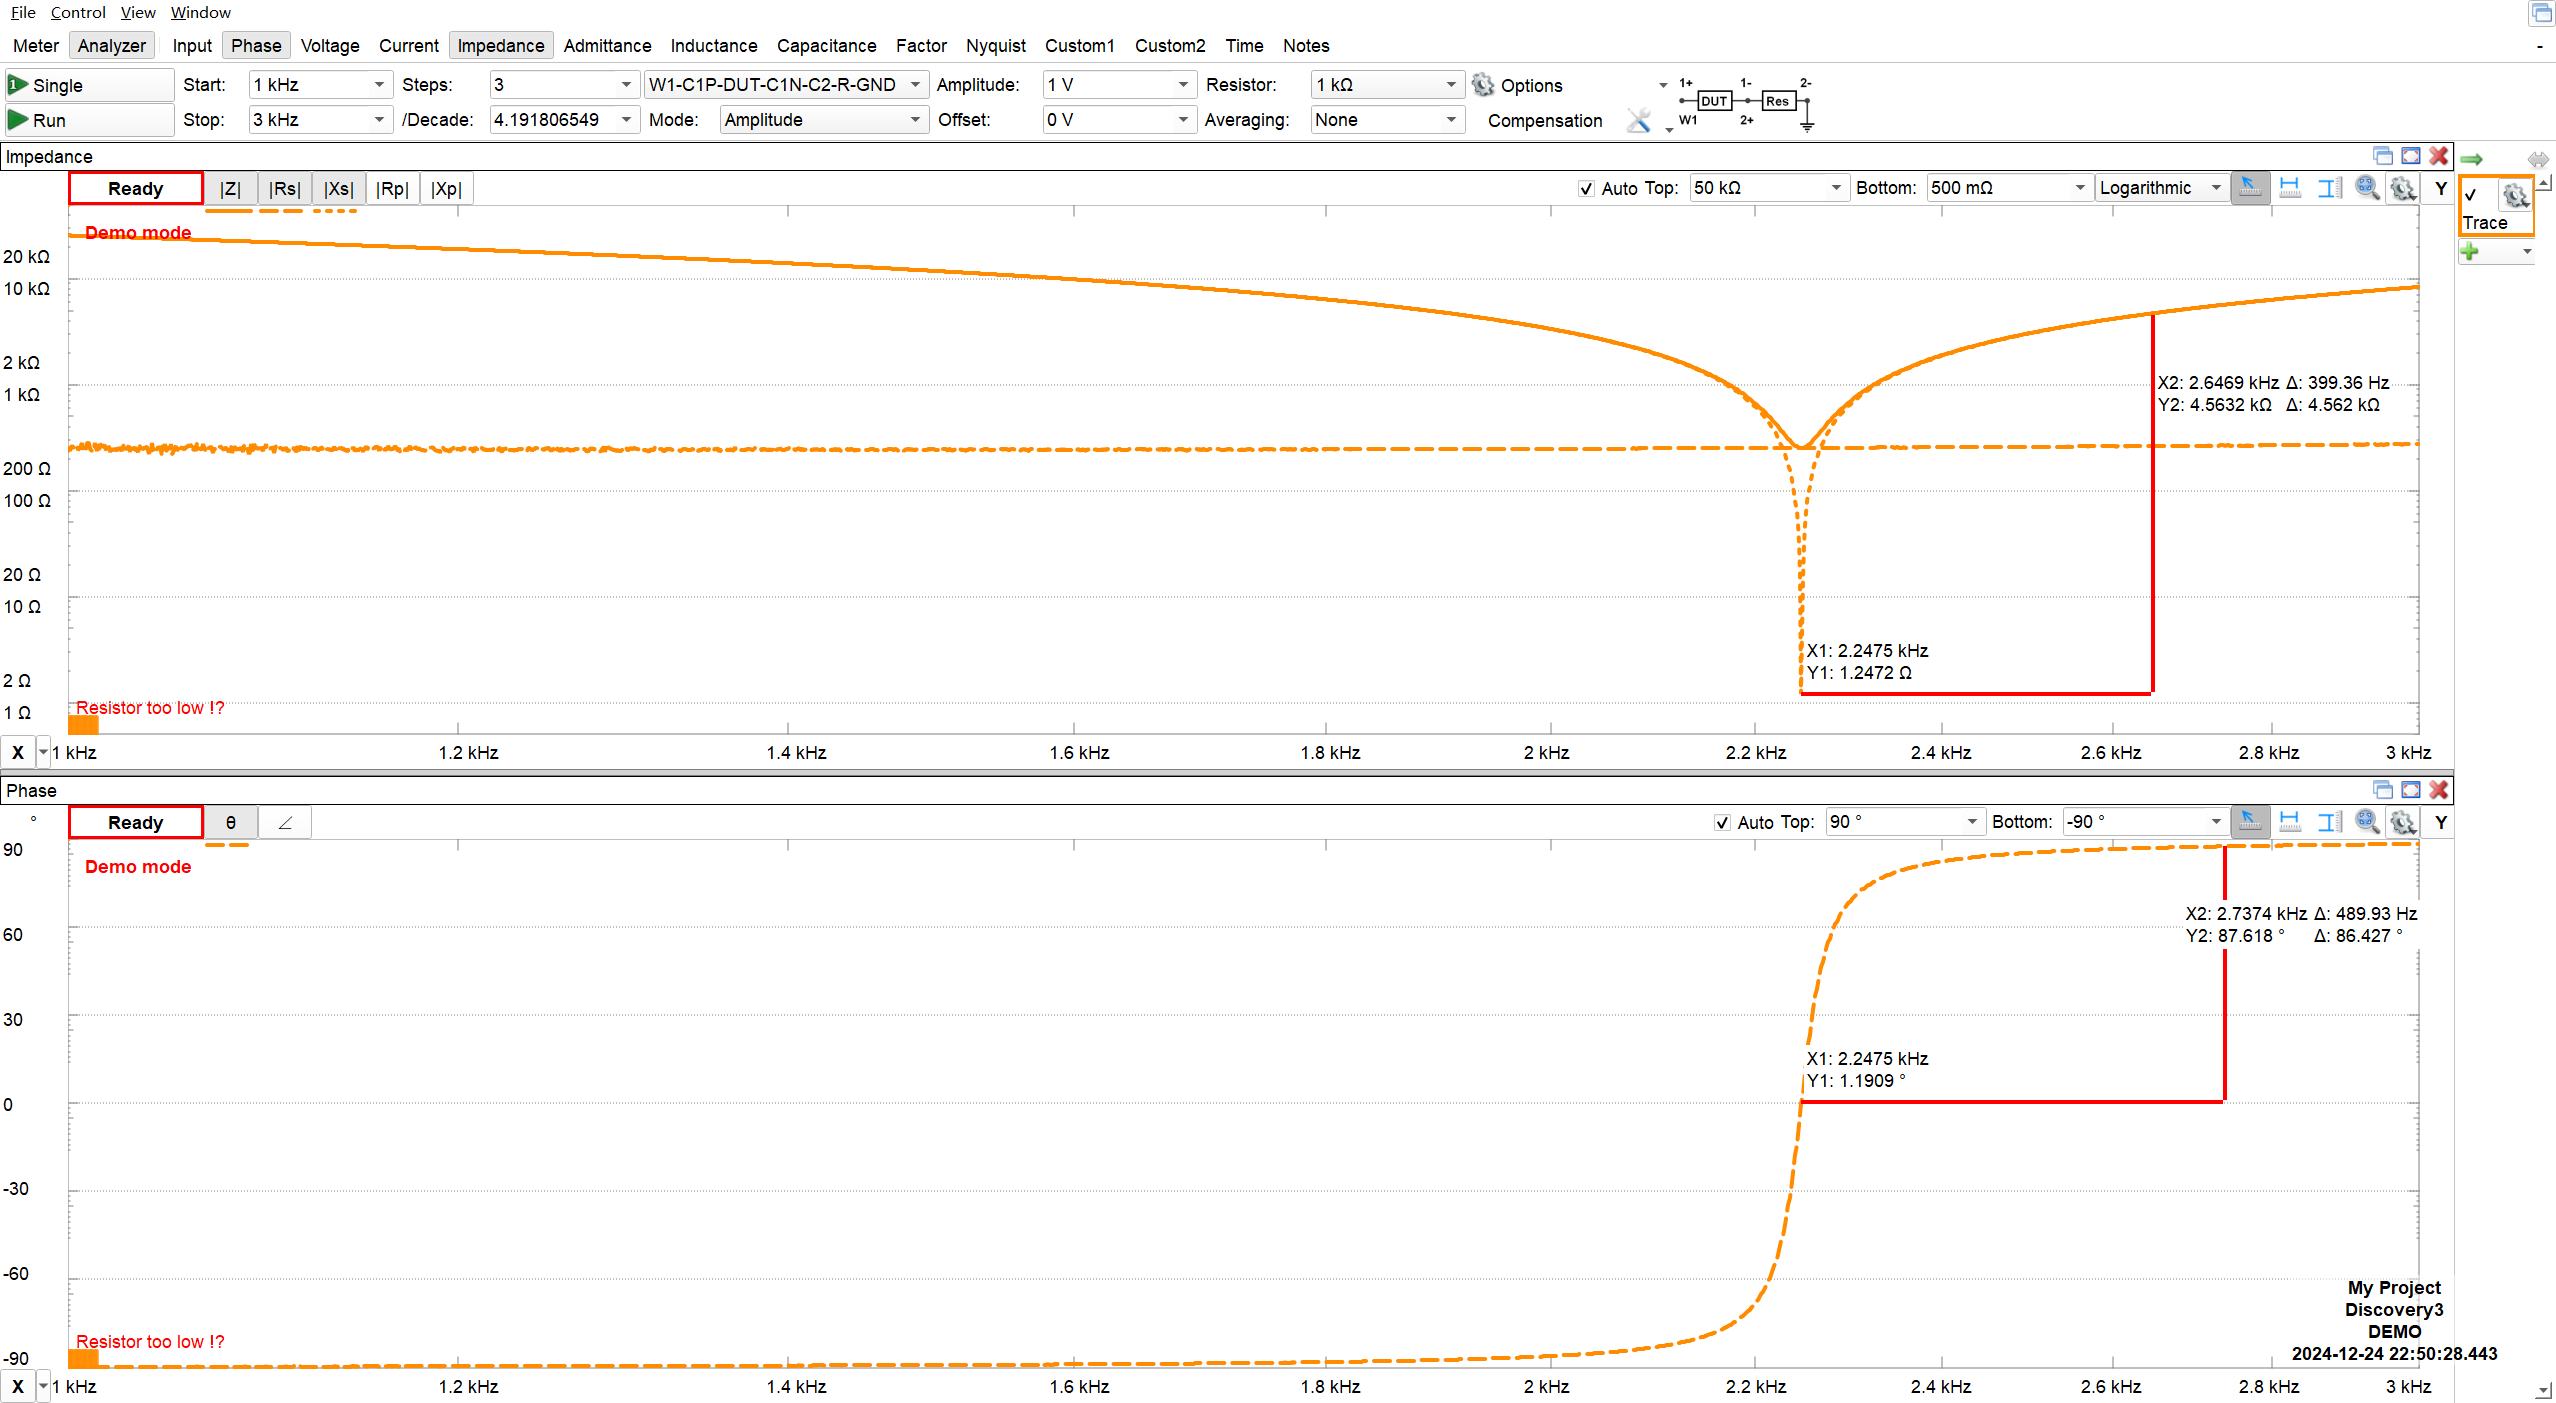
\includegraphics[width=\columnwidth]{assets/1/20241224 RLC 实验, RLC 串联, 阻抗曲线.png}
    \caption{AD1 设备测得的 $RLC$ 串联电路阻抗与相位曲线 $(f \in [1 \ \mathrm{KHz},\ 3 \ \mathrm{KHz}])$}
\end{figure}
可以看到,谐振频率约为 $2.2475 \ \mathrm{KHz}$,与前面的结果基本吻合。


\subsection{测$ RLC $并联电路的相频特性和幅频特性曲线}

先调节函数发生器输出频率至并联部分电压$ u $与总电流相位相同,即达到谐振,此时可得谐振频率为
\begin{equation}
f_p=2.2472\,\mathrm{kHz}
\end{equation}

然后在参考频率下测得实验数据如表 \ref{RLC 并联谐振电路实验数据记录}。

\begin{table}[H]\centering
    %\renewcommand{\arraystretch}{1.5} % 调整行间距为 1.5 倍
    %\setlength{\tabcolsep}{1.5mm} % 调整列间距
    \caption{$ RLC $并联谐振电路实验数据记录}
    \label{RLC 并联谐振电路实验数据记录}
\begin{tabular}{cccccccccc}\toprule
    $f$ (KHz) & $U_{\text{amp}}$ (V) & $\Delta t$ (us) & $\varphi$ ($^\circ$) & $U_{ \text{amp}}$ (V)  & $U_{R, \text{amp}}$ (mV) & $I_{\max}$ (mA)  \\
    \midrule
    2.050	&2.00	&105	&77.490	    &1.52	&912	    &182.4  \\
    2.150	&2.00	&97	    &75.078	    &1.75	&480	    &96.0   \\
    2.200	&2.00	&83	    &65.736	    &1.79	&286	    &57.2   \\
    2.231	&2.00	&52	    &41.764	    &1.82	&134	    &26.8   \\
    2.240	&2.00	&12	    &9.677	    &1.79	&96	        &19.2   \\
    2.247	&2.00	&1	    &0.809	    &1.82	&108	    &21.6   \\
    2.250	&2.00	&-14	&-11.340	&1.80	&114	    &22.8   \\
    2.253	&2.00	&-21	&-17.033	&1.79	&119	    &23.8   \\
    2.256	&2.00	&-31	&-25.177	&1.78	&121	    &24.2   \\
    2.265	&2.00	&-57	&-46.478	&1.75	&137	    &27.4   \\
    2.275	&2.00	&-93	&-76.167	&1.74	&175	    &35.0   \\
    2.320	&2.00	&-95	&-79.344	&1.67	&411	    &82.2   \\
    2.400	&2.00	&-99	&-85.536	&1.32	&762	    &152.4  \\
    2.600	&2.00   &-101   &-94.536	&1.11	&1290	    &258.0  \\
    \bottomrule 
\end{tabular}
\end{table}

其中,示波器光标功能仅能读取相同相位点间的时间间隔,根据$ \Delta t $计算相位差$ \varphi $的公式为
\begin{equation}
\varphi=2\pi f\Delta t
\end{equation} 

根据表 \ref{RLC 并联谐振电路实验数据记录} 数据可作出图 \ref{RLC 并联电路频率响应}。
\begin{figure}[H]\centering
\begin{subfigure}[b]{0.33\columnwidth}\centering
    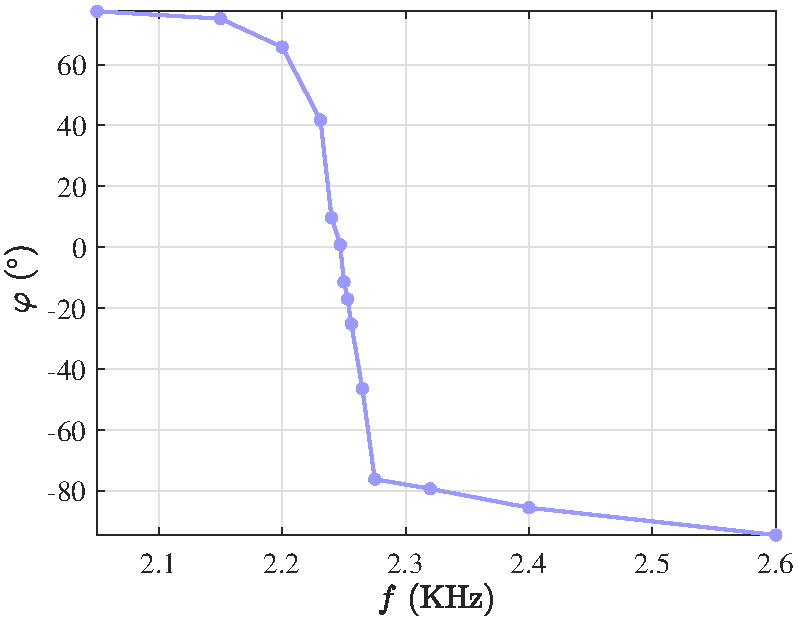
\includegraphics[height=125pt]{assets/2/2024-12-24_22-29-02.pdf}
    \caption{相位 $\varphi$}
\end{subfigure}\hfill
\begin{subfigure}[b]{0.33\columnwidth}\centering
    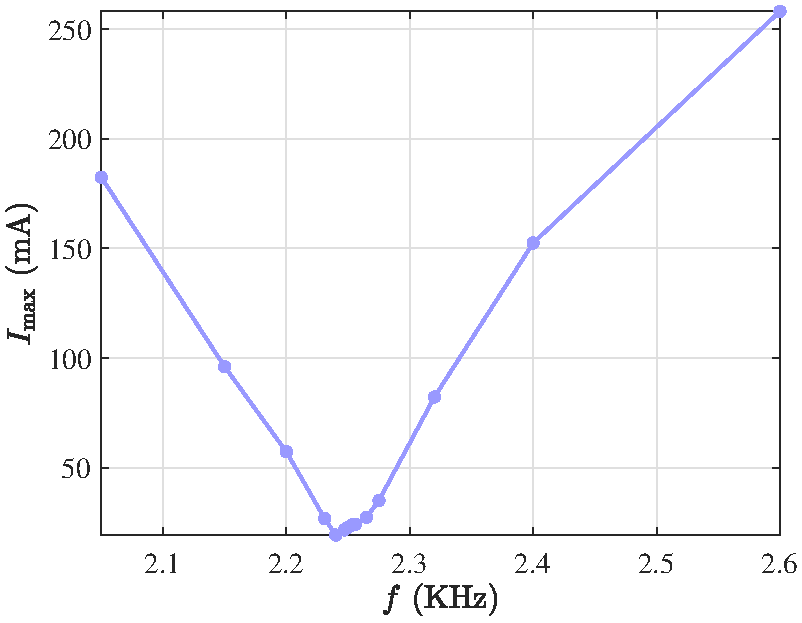
\includegraphics[height=125pt]{assets/2/2024-12-24_22-29-05.pdf}
    \caption{电流 $I_{\max}$}
\end{subfigure}
\begin{subfigure}[b]{0.33\columnwidth}\centering
    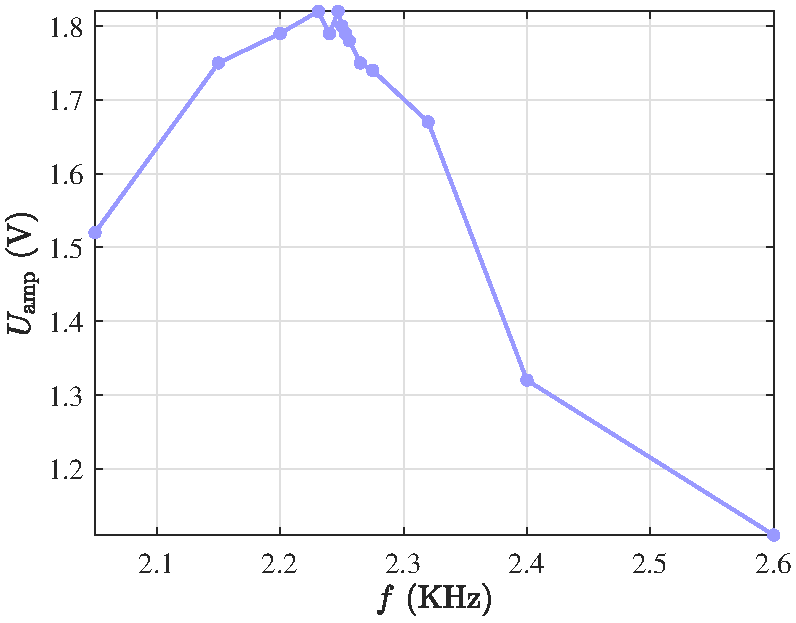
\includegraphics[height=125pt]{assets/2/2024-12-24_22-29-08.pdf}
    \caption{电压 $U_{\text{amp}}$}
\end{subfigure}
\caption{$RLC$ 并联电路频率响应}
\label{RLC 并联电路频率响应}
\end{figure}

AD1 设备测得的阻抗与相位曲线如图 \ref{RLC 并联电路阻抗与相位曲线} 所示:
\begin{figure}[H]\centering
    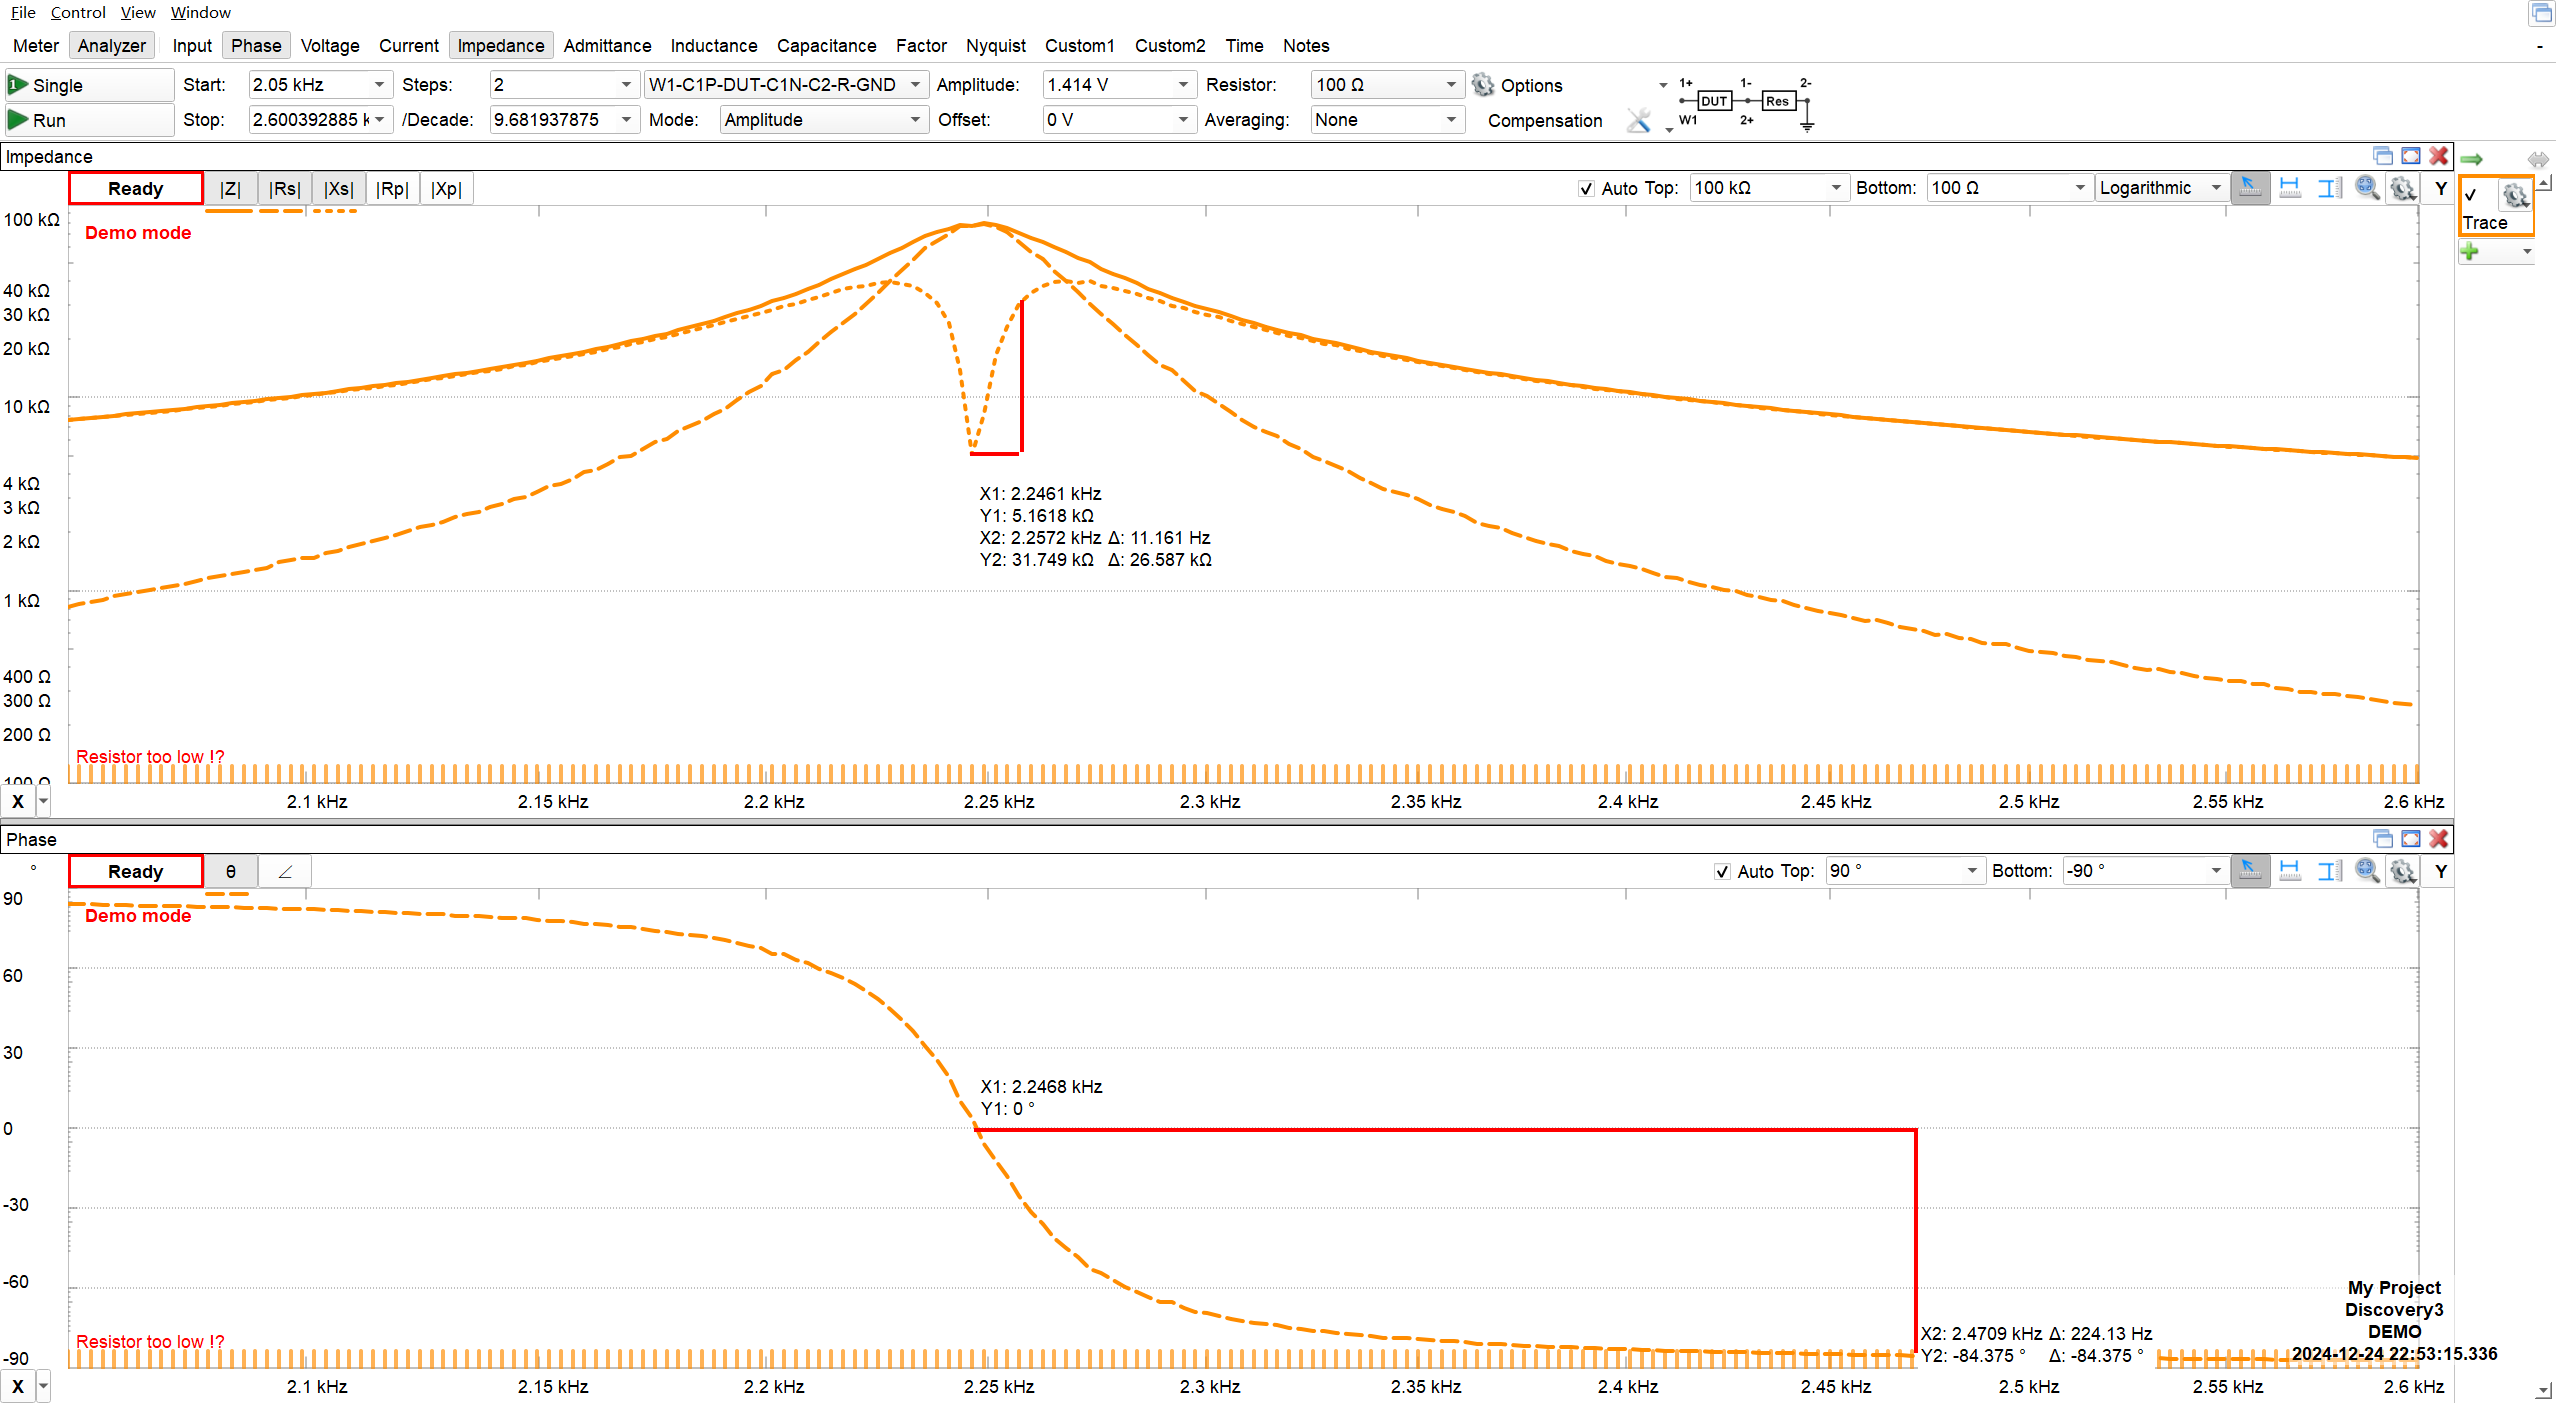
\includegraphics[width=\columnwidth]{assets/2/20241224 RLC 实验, RLC 并联, 阻抗曲线.png}
    \caption{AD1 设备测得 $RLC$ 并联电路的阻抗与相位曲线 $(f \in [2 \ \mathrm{KHz},\ 2.6 \ \mathrm{KHz}])$}
    \label{RLC 并联电路阻抗与相位曲线}
\end{figure}


\subsection{观测$ RLC $串联电路的暂态过程}

类似地,这一小节我们也同时使用示波器和 AD1 去观测 $RLC$ 串联电路的暂态过程,如图 \ref{AD1 RLC 串联电路暂态过程}。
\begin{figure}[H]\centering
    \includegraphics[width=\columnwidth]{assets/3/d03b86529721f8b11761bef084cea7e8.png}
    \caption{同时使用示波器和 AD1 观测 $RLC$ 串联电路的暂态过程}
    \label{AD1 RLC 串联电路暂态过程}
\end{figure}


\subsubsection{欠阻尼 ($ 50\ \mathrm{Hz}, 0 \ \Omega$)}

调节$ R=0\,\Omega $,$f = 50$ Hz,得到$ u_C $波形如下:
\begin{figure}[H]\centering
    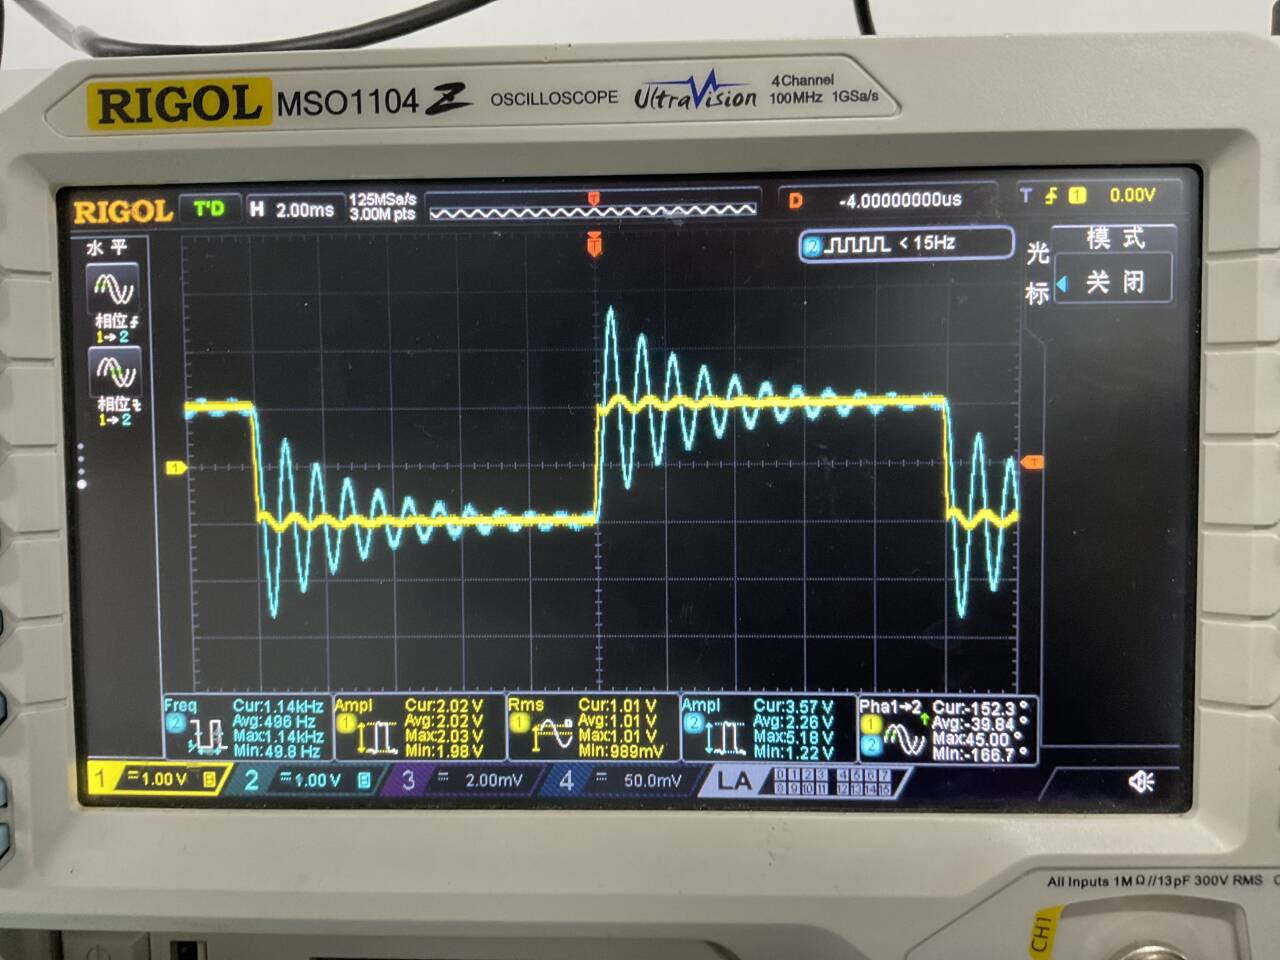
\includegraphics[width=0.9\columnwidth]{assets/3/0f8c992ad87b9eae1916428d4d32a128_720.png}
    \caption{欠阻尼波形 (示波器)}
\end{figure}

\begin{figure}[H]\centering
    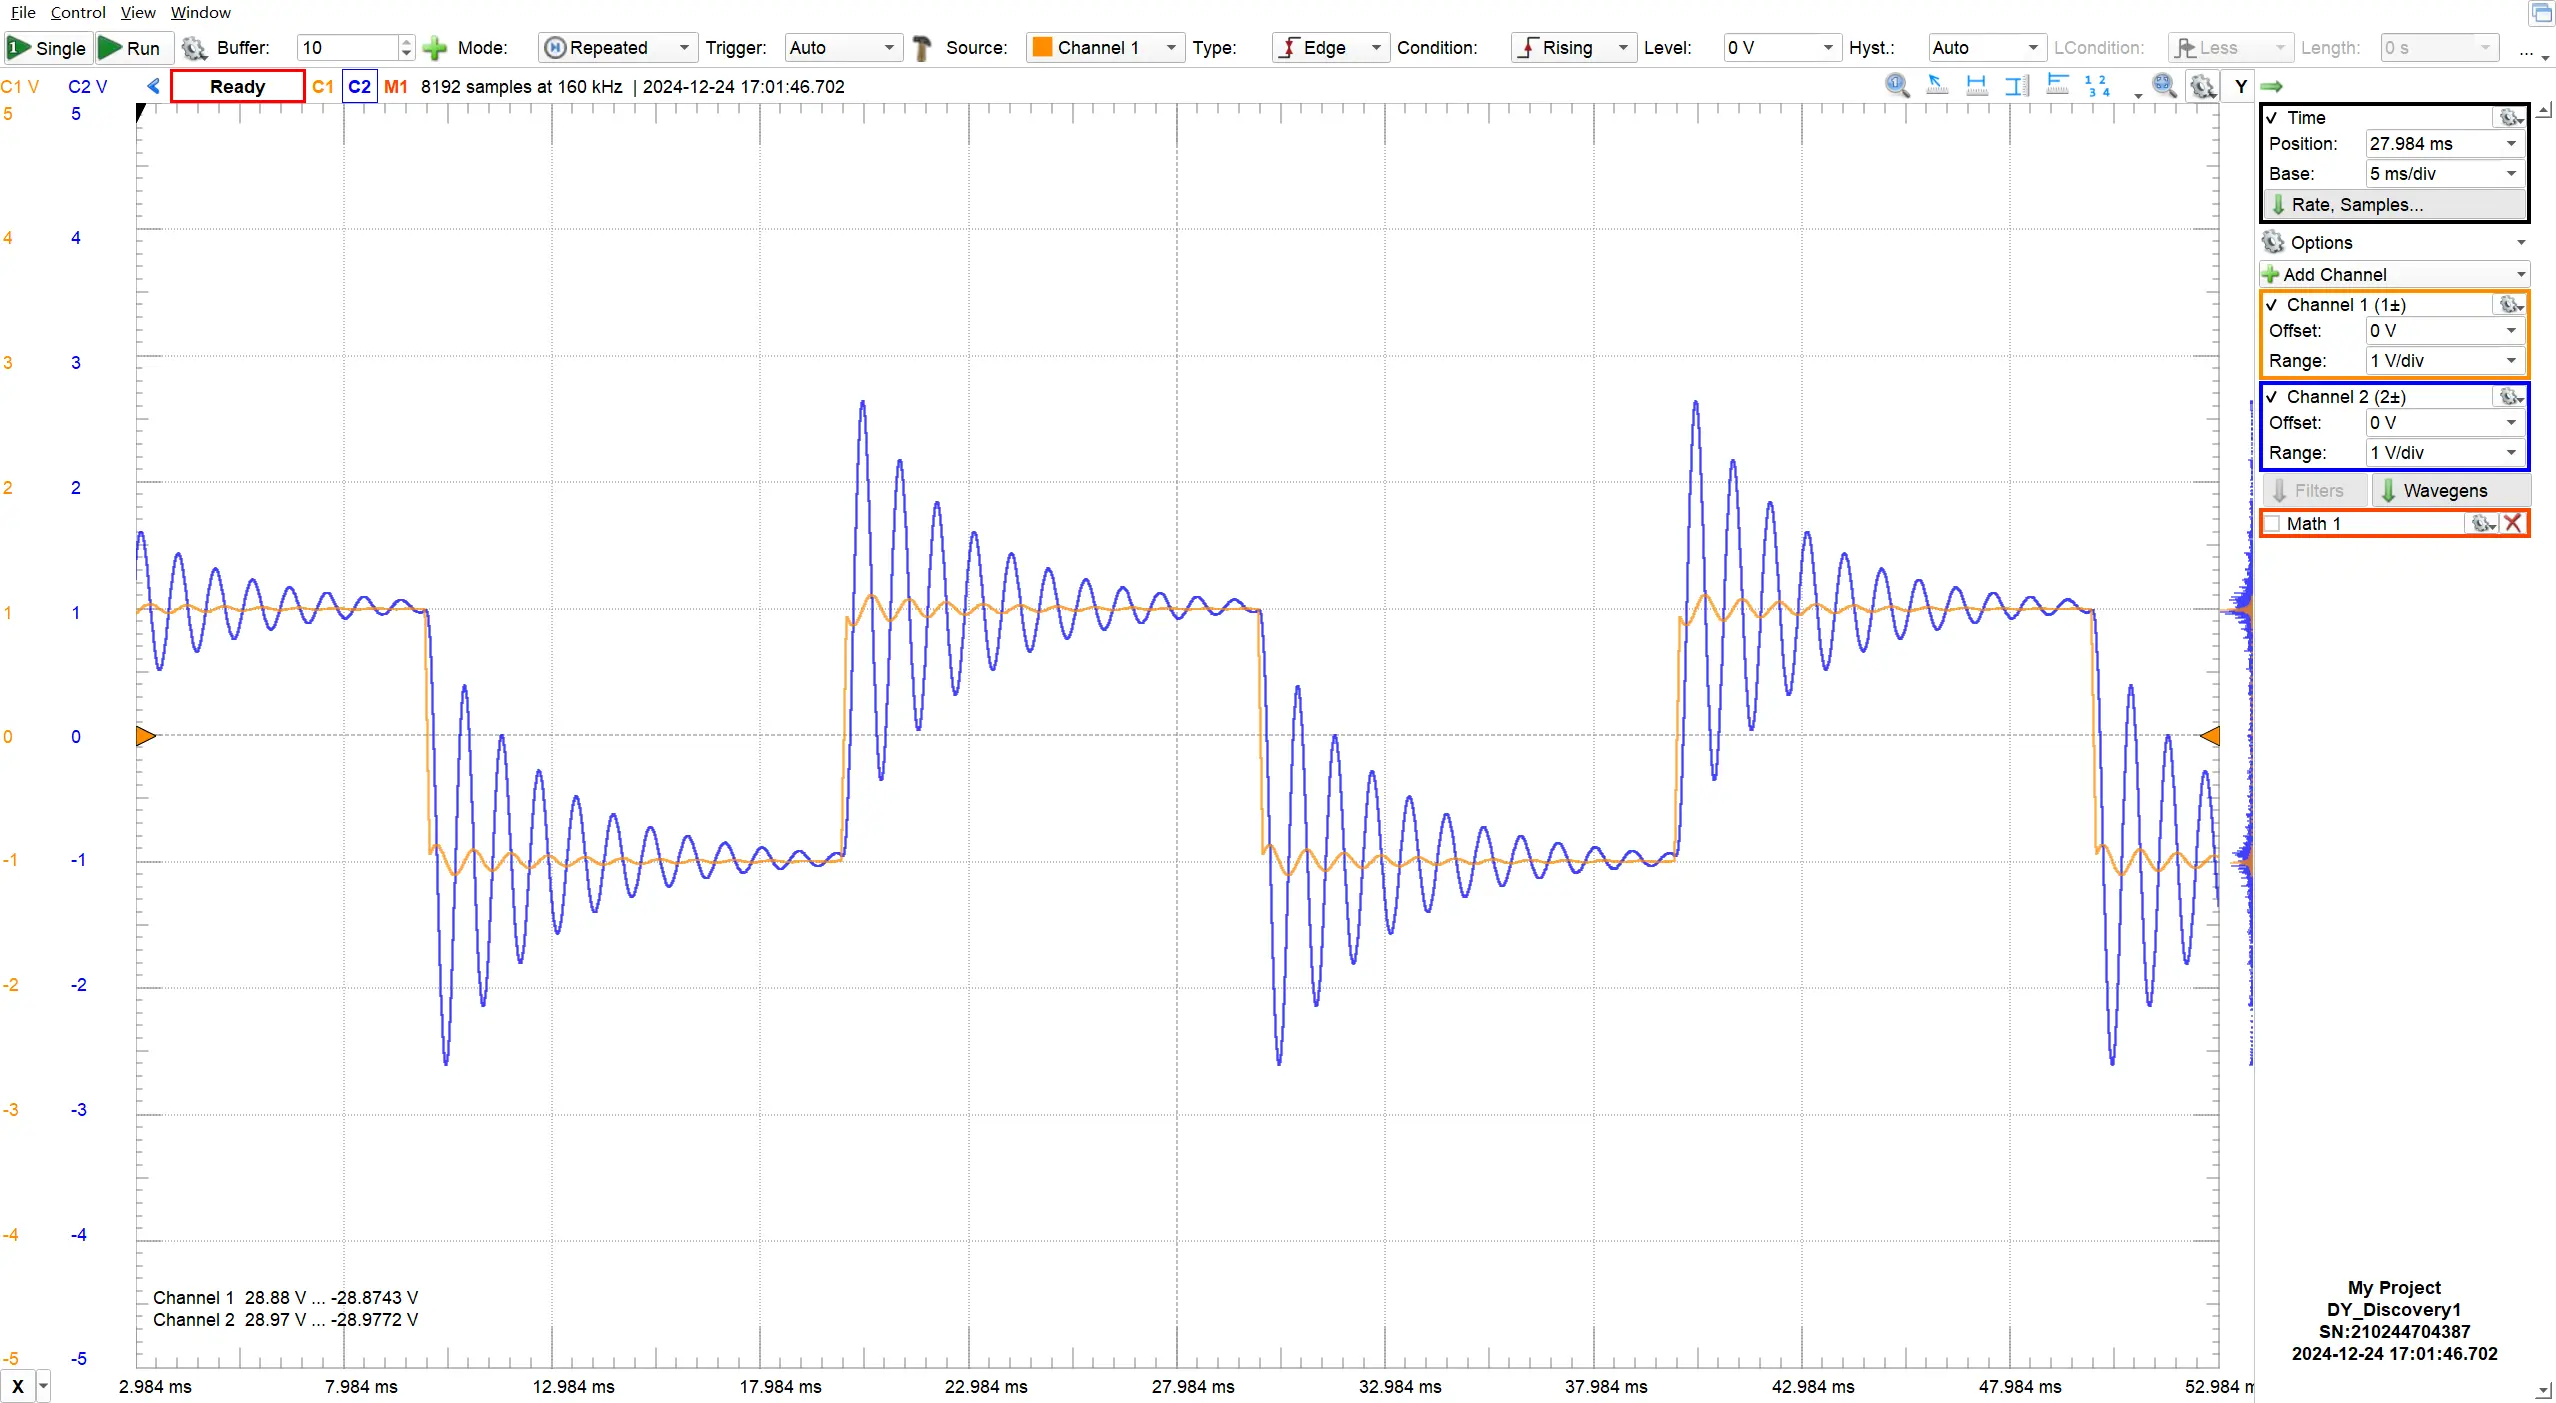
\includegraphics[width=0.9\columnwidth]{assets/3/20241224 RLC 实验, RLC 暂态, 50Hz 0 Ohm 欠阻尼.png}
    \caption{欠阻尼波形 (AD1)}
\end{figure}

\subsubsection{临界阻尼 ($ 50\ \mathrm{Hz}, 1410 \ \Omega$)}

自小到大调节$ R $的大小,当$ R=1410\,\Omega $时,波形振动几乎消失,可近似看作临界阻尼状态,波形如下:
\begin{figure}[H]\centering
    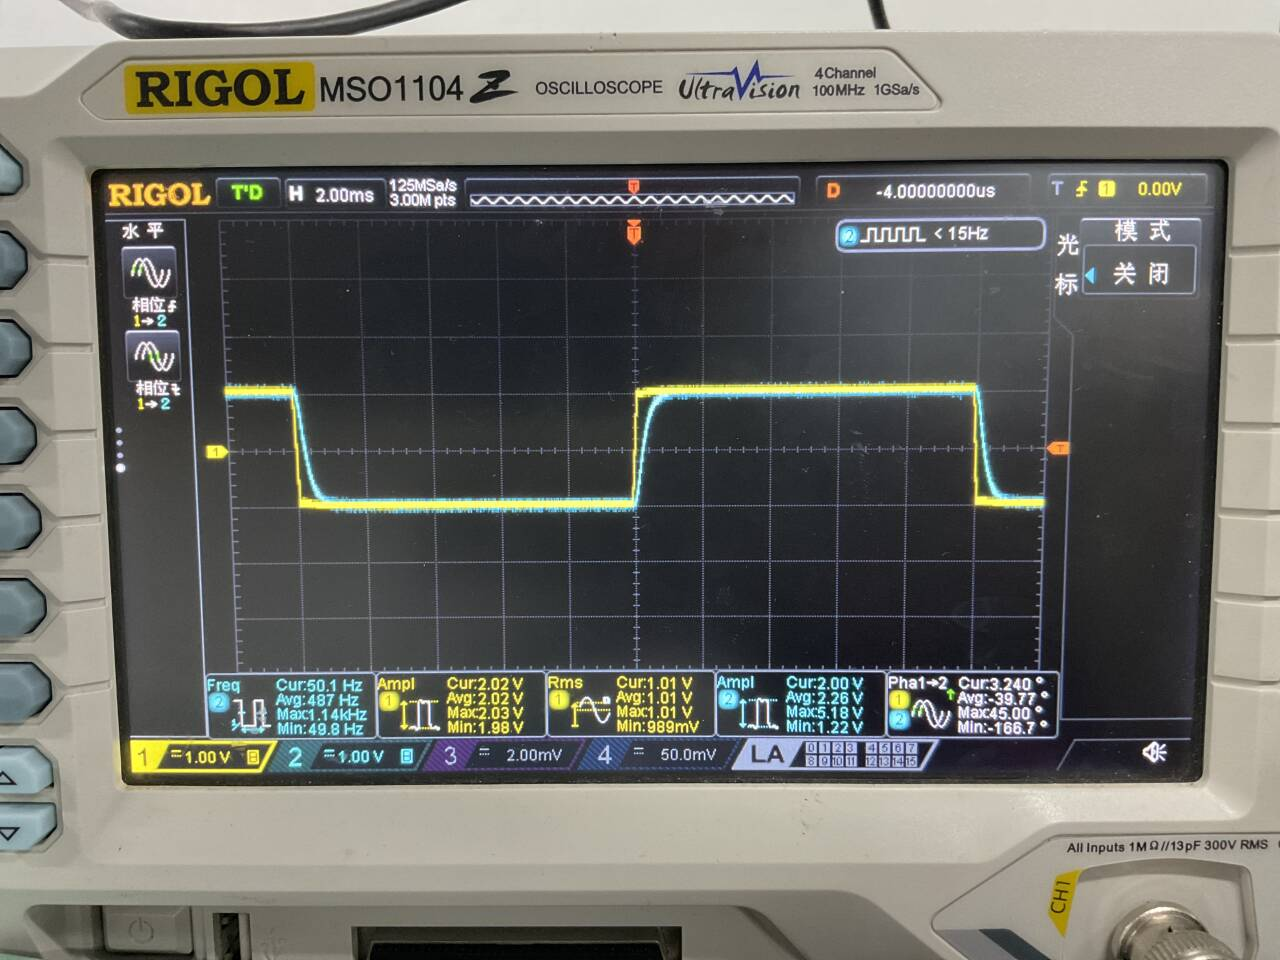
\includegraphics[width=0.9\columnwidth]{assets/3/de9a909a297bc9eb880b069c61728fab_720.png}
    \caption{临界阻尼波形 (示波器)}
\end{figure}

根据实验所用电路元件参数可计算得到临界电阻理论值$ R_C $为 $R_C=\sqrt{\frac{4L}{C}}\approx1414\,\Omega$,与实际测得的结果较为接近。存在误差是因为临界阻值附近波形不明显,以及电路中电感电容存在内阻。

\begin{figure}[H]\centering
    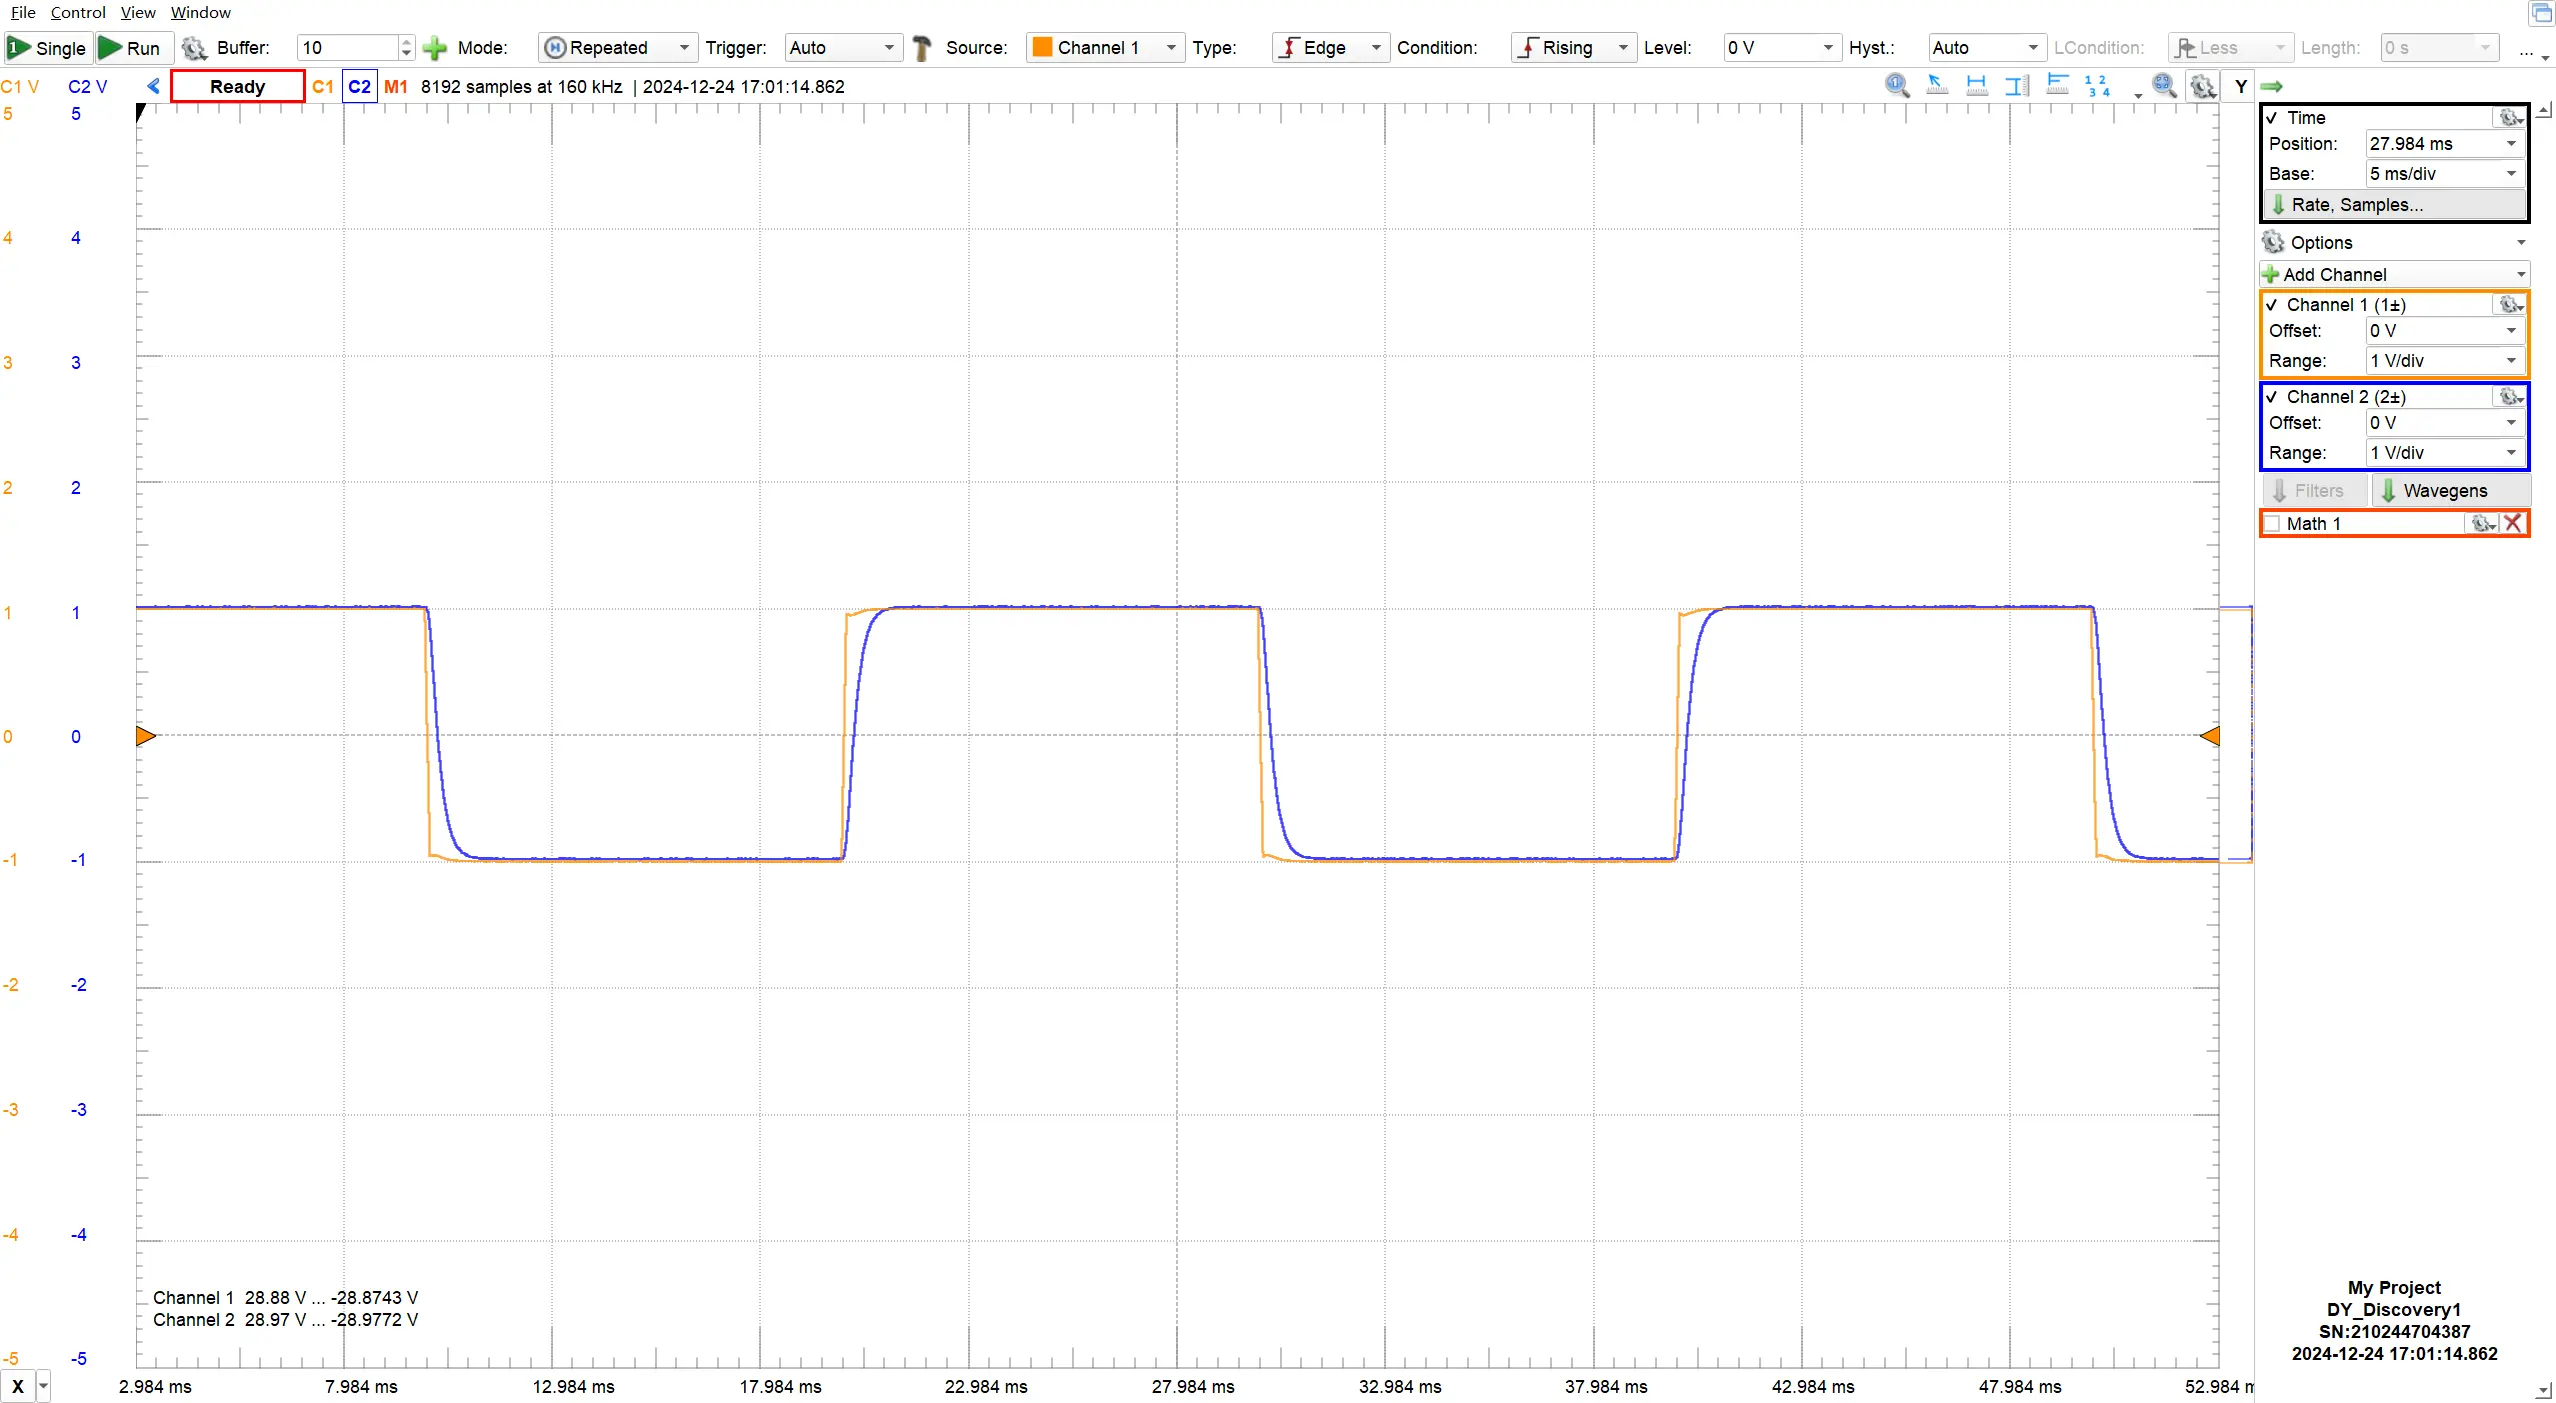
\includegraphics[width=0.9\columnwidth]{assets/3/20241224 RLC 实验, RLC 暂态, 50Hz 1410 Ohm 临界阻尼.png}
    \caption{临界阻尼波形 (AD1)}
\end{figure}

\subsubsection{过阻尼 (50 Hz, 20 $\KO$)}


调节$ R $至过阻尼状态,在相应频率下记录$ u_C $波形:
\begin{figure}[H]\centering
    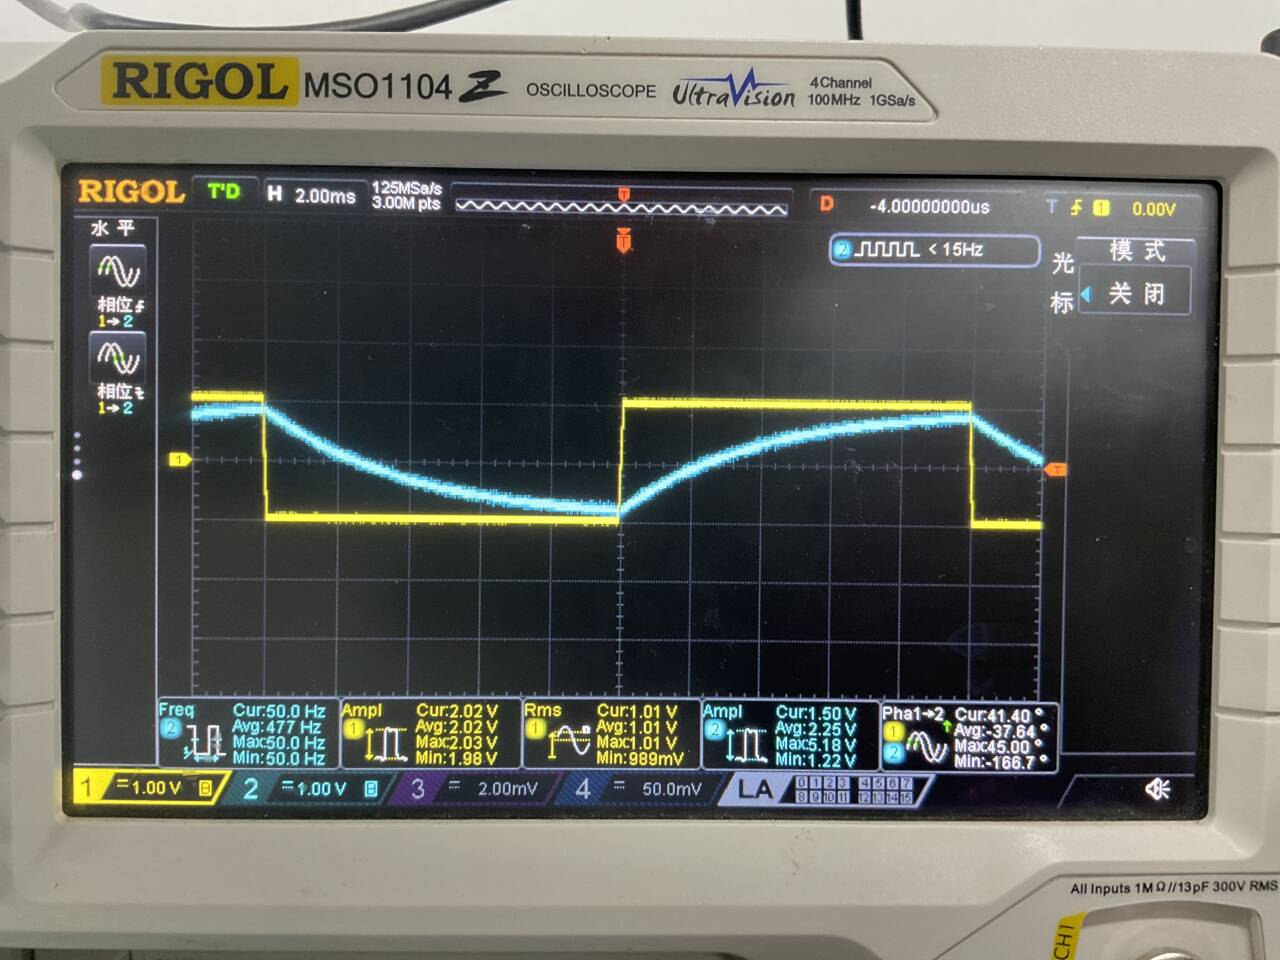
\includegraphics[width=0.9\columnwidth]{assets/3/2c252ca3fcad60a9e464d10f86af03e1_720.png}
    \caption{过阻尼波形 (示波器)}
\end{figure}

\begin{figure}[H]\centering
    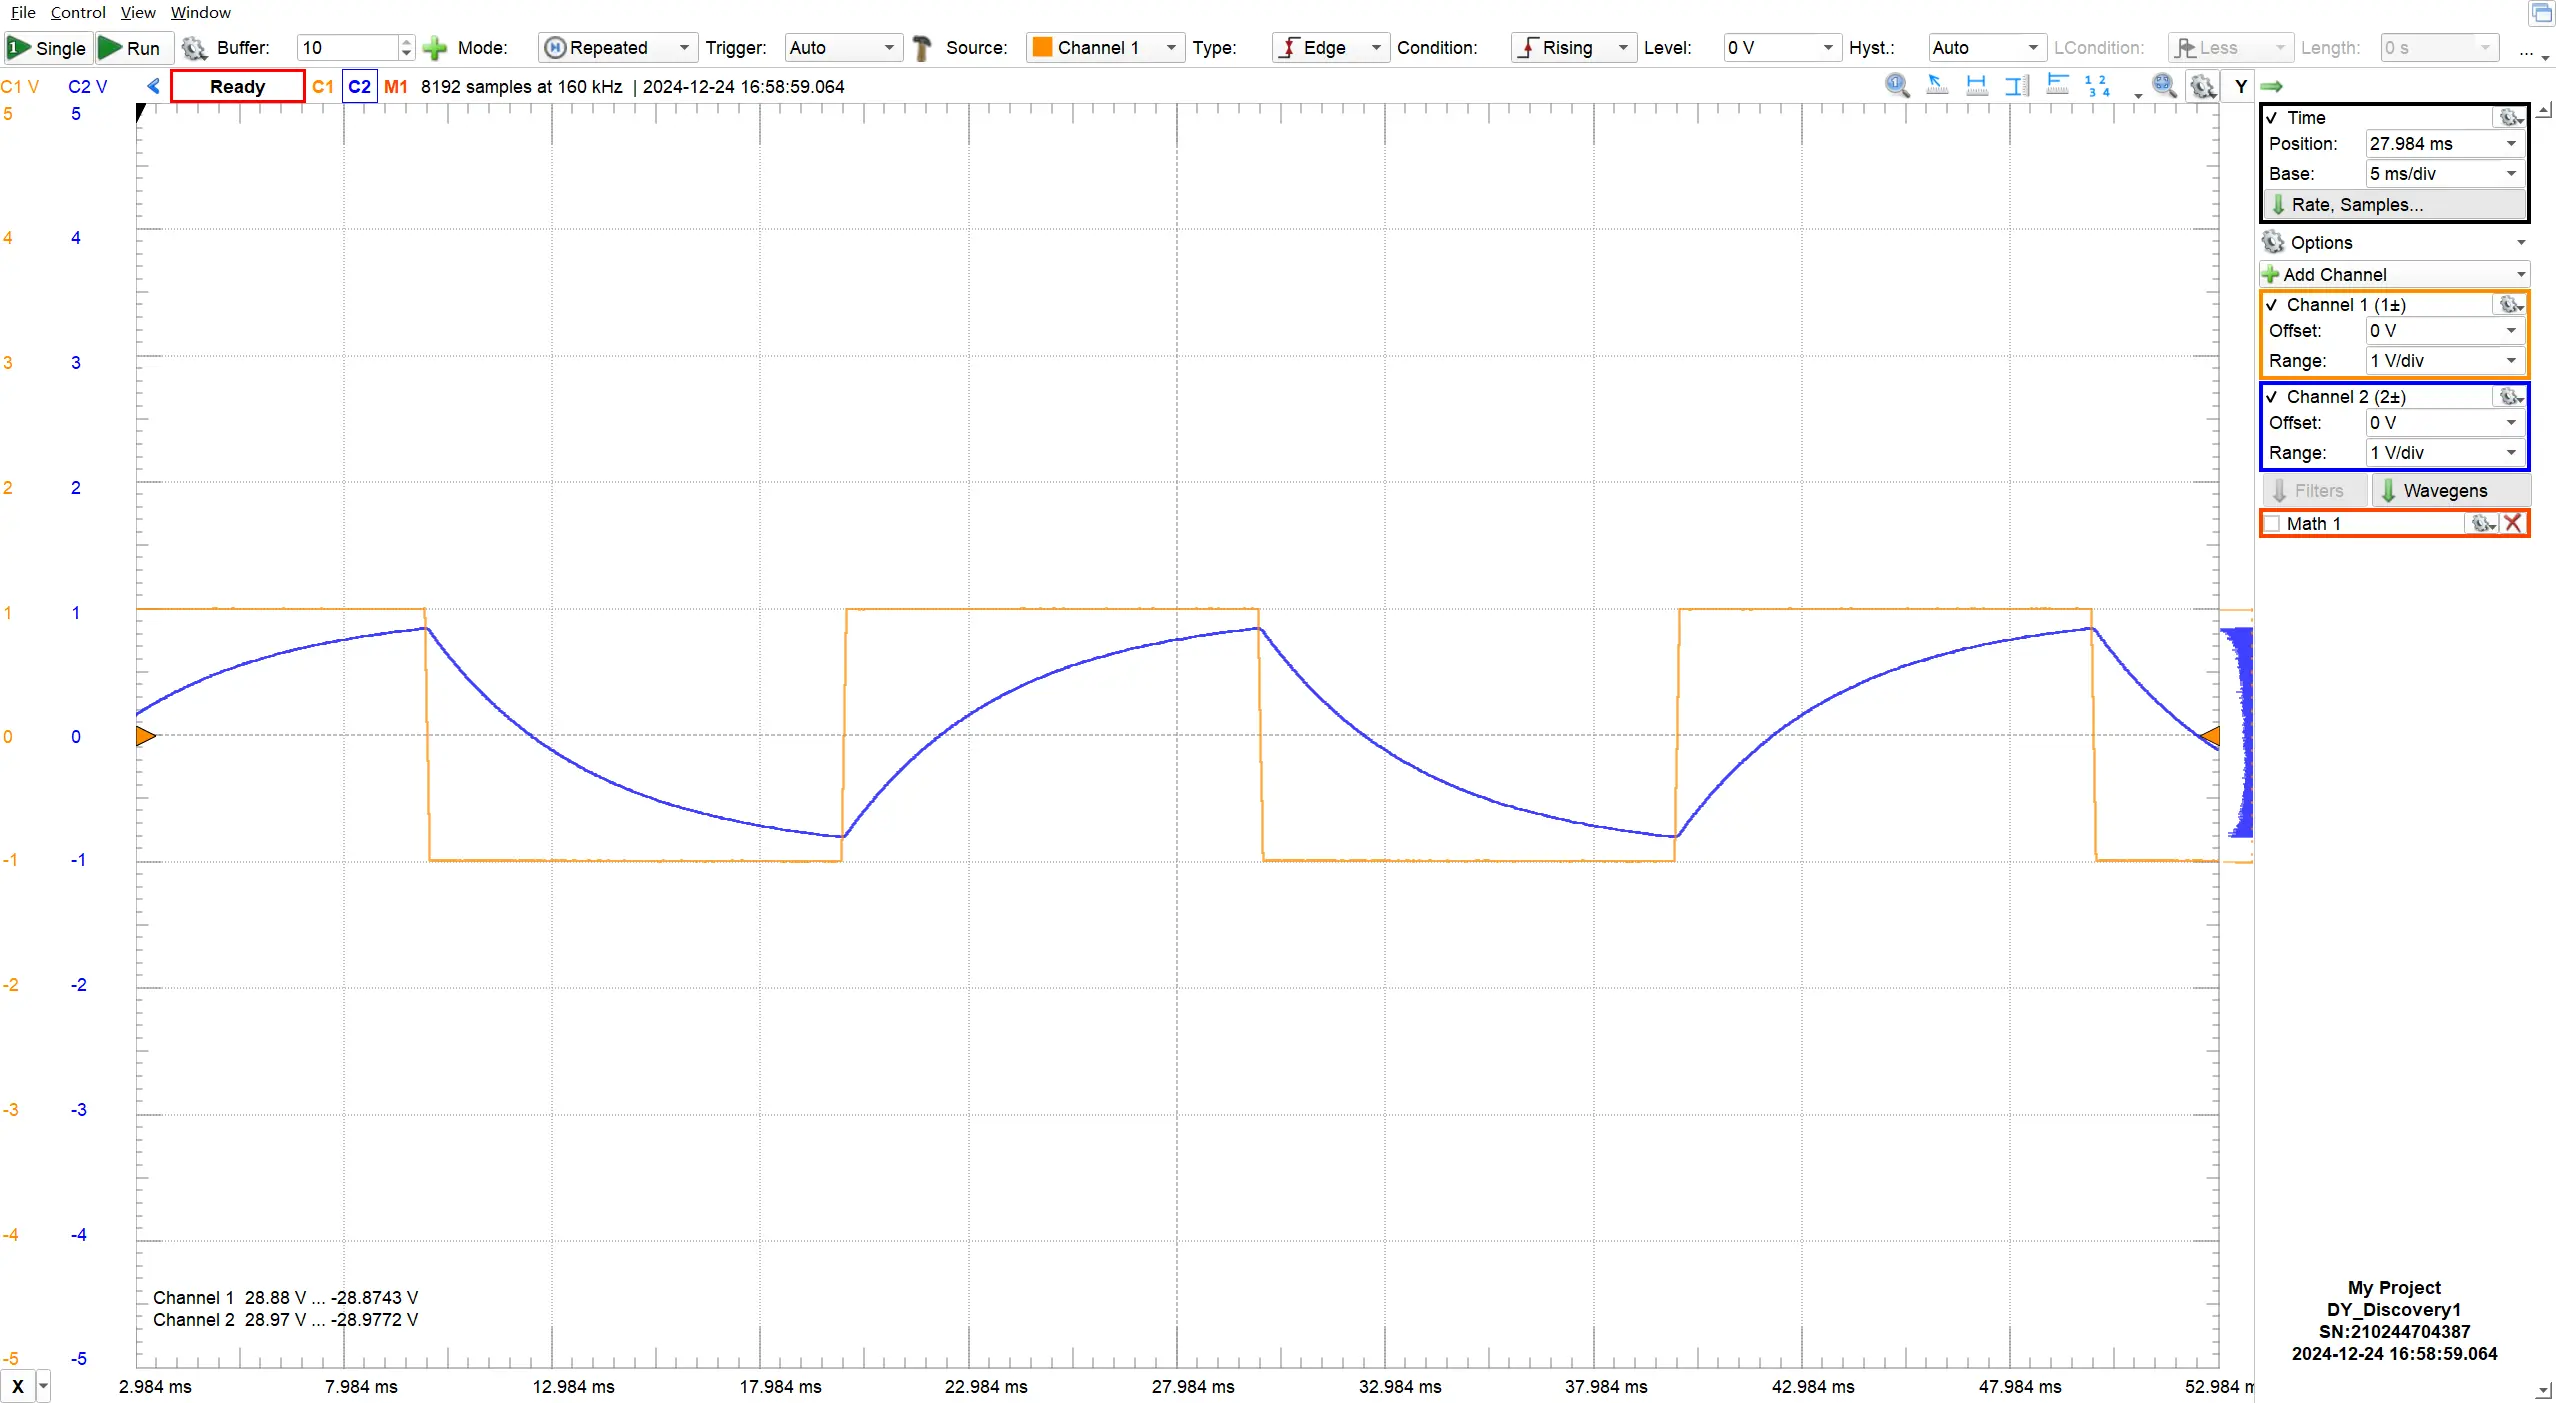
\includegraphics[width=0.9\columnwidth]{assets/3/20241224 RLC 实验, RLC 暂态, 50Hz 20K Ohm 过阻尼.png}
    \caption{过阻尼波形 (AD1)}
\end{figure}

\section{实验总结与心得体会}

此次“$RLC$ 谐振实验”实验共分为三个部分,分别是串联谐振、并联谐振和暂态过程,实验步骤均比较简单,但需要注意的细节很多。实验的一个要点是“示波器共地”,若不注意共地现象,很容易造成短路,轻则无法继续实验,重则损坏实验设备甚至产生安全隐患。我自己也尝试了示波器共地和不共地的两种情况,不共地时确实无法正常测量,因此印象深刻;另一重点是数据的记录与计算,在处理的过程中,我也学到很多。实验总体上是成功的,每个小节的实验都大致符合理论,实验数据和图像也具有较强的说服力。

特别地,在本次实验,我利用了 Digilent 生产的 Analog Discovery 1 设备。它是一种 all-in-one 的可编程多功能设备,用官方的话来说就是 "It is a multi-function programmable instrument that allows users to measure, visualize, generate, record, and control mixed signal circuits of all kinds"。对于我们电子信息工程专业的学生来讲,以后少不了和模拟电路、数字电路打交道,设计、调试电路也会成为常态。因此,学会使用像这样集成了多种功能、可编程的、能够将重复性测量流程自动化的设备,能够大大提高我们开发、测试元件和电路的效率。本次实验就是一个最典型的例子,测量 $RLC$ 串联电路的谐振频率时我们花了约一小时,而通过编程控制 AD1 进行测量,只需要 5s 至 20s 就可以得到结果,并且精度极高,效率极大地提高了。因此,我认为学习并利用可编程设备是非常有益,它能够帮助我们更好地学习和研究电路,提高我们的实验和创新能力。

另外,我还使用了 Matlab 软件对实验数据作进一步的处理和分析,包括计算和可视化等,相比于常规数据处理和画图方法,这大大提高了数据分析处理的速度的准确度,也提高了作图的美观性。在今后的实验和研究工作中,我还会继续深入学习和应用类似地计算软件,增强自己的科学计算能力。科研不是考试,我们应该充分利用好自己能接触到的资源,合理使用工具,更高效地发展自身。

另外,这次实验让我感受到,实验“结束”并不意味着实验就已经完成,事实上这仅是数据测量的结束。在课后,我们还需要重新整理实验原理和过程,换算、分析、拟合实验数据,作出合适的数据图,解释可能存在的误差等。在根据已有数据求所需结果时,如何才能最大程度地利用已有数据,同时又尽可能地降低二次误差。上面这些内容都需要体现在最终的实验报告中,一点点累加起来,着实花费了我很多精力。

最后回过头来,我认为一切都是值得的。当处理完毕的结果有力地验证了理论值时,当实验数据图像与理论较好地契合时,心中便迸发出无尽的喜悦,也深深感受到物理“理论与实验结合”的魅力\footnote{本次实验的预习报告是撰写实验报告的前半部分,内容是重复的,因此不再给出;实验数据记录表和 Matlab 源码附在附录中}。


\newpage
\subsection*{附录 A\hspace*{20pt} 原始数据记录表}
\addcontentsline{toc}{section}{附录 A\hspace*{6pt} 原始数据记录表} 
\thispagestyle{fancy} 

\begin{figure}[H]\centering
    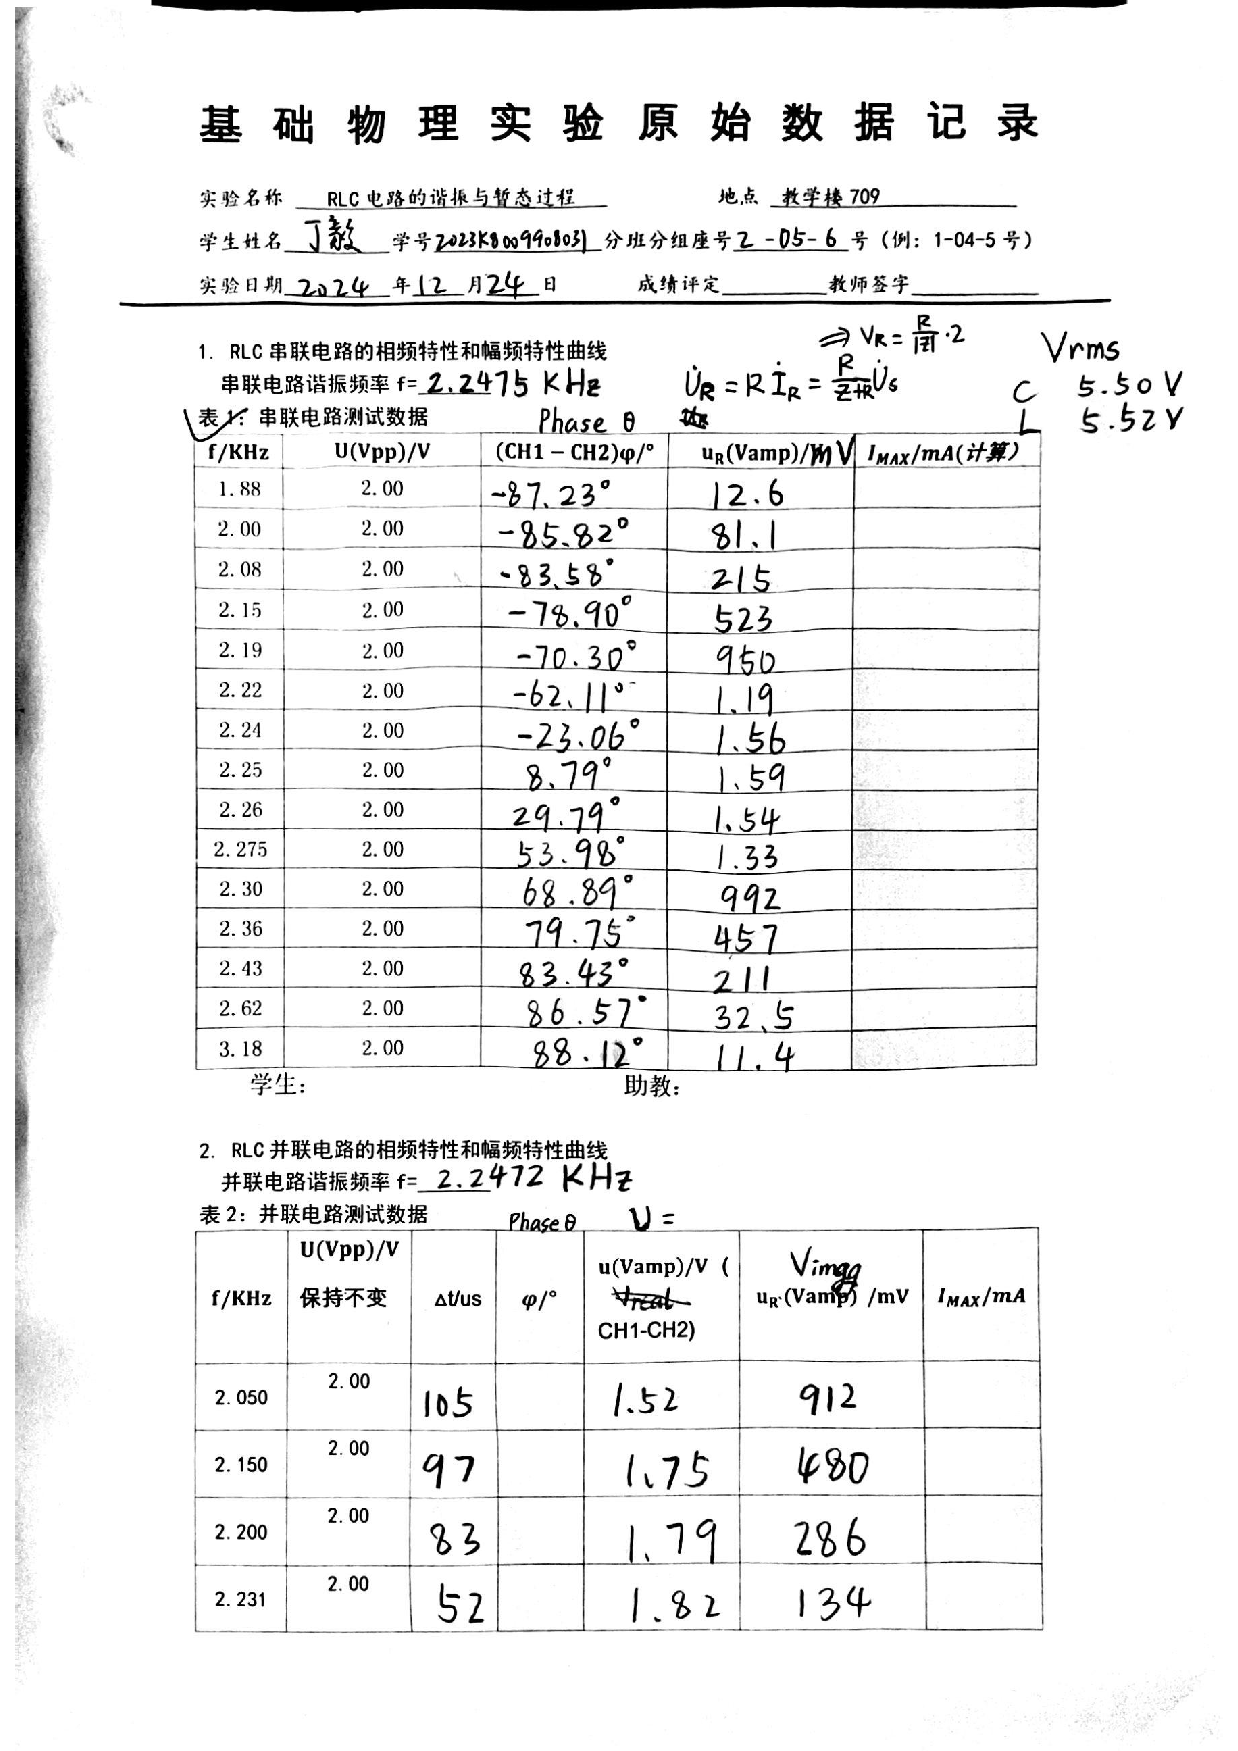
\includepdf[pages=1, width=480pt]{pdf/原始数据-2-05组-丁毅-谐振电路-2024.12.24-邓体建.pdf}
\end{figure}
\includepdf[pages={2}]{pdf/原始数据-2-05组-丁毅-谐振电路-2024.12.24-邓体建.pdf}

\subsection*{附录 B\hspace*{20pt} Matlab 源码}
\addcontentsline{toc}{section}{附录 B\hspace*{6pt} Matlab 源码} 
\thispagestyle{fancy} 
\lstinputlisting{d:/a_RemoteRepo/GH.MatlabCodes/本科课程代码/基础物理实验/Ex_6/Ex_06_mfile.m}




\end{document}

% VScode 常用快捷键:

% F2:                       变量重命名
% Ctrl + Enter:             行中换行
% Alt + up/down:            上下移行
% 鼠标中键 + 移动:           快速多光标
% Shift + Alt + up/down:    上下复制
% Ctrl + left/right:        左右跳单词
% Ctrl + Backspace/Delete:  左右删单词    
% Shift + Delete:           删除此行
% Ctrl + J:                 打开 VScode 下栏(输出栏)
% Ctrl + B:                 打开 VScode 左栏(目录栏)
% Ctrl + `:                 打开 VScode 终端栏
% Ctrl + 0:                 定位文件
% Ctrl + Tab:               切换已打开的文件(切标签)
% Ctrl + Shift + P:         打开全局命令(设置)

% Latex 常用快捷键:

% Ctrl + Alt + J:           由代码定位到PDF


